\PassOptionsToPackage{unicode=true}{hyperref} % options for packages loaded elsewhere
\PassOptionsToPackage{hyphens}{url}
%
\documentclass[12pt,]{article}
\usepackage{lmodern}
\usepackage{amssymb,amsmath}
\usepackage{ifxetex,ifluatex}
\usepackage{fixltx2e} % provides \textsubscript
\ifnum 0\ifxetex 1\fi\ifluatex 1\fi=0 % if pdftex
  \usepackage[T1]{fontenc}
  \usepackage[utf8]{inputenc}
  \usepackage{textcomp} % provides euro and other symbols
\else % if luatex or xelatex
  \usepackage{unicode-math}
  \defaultfontfeatures{Ligatures=TeX,Scale=MatchLowercase}
    \setmainfont[]{Minion Pro}
\fi
% use upquote if available, for straight quotes in verbatim environments
\IfFileExists{upquote.sty}{\usepackage{upquote}}{}
% use microtype if available
\IfFileExists{microtype.sty}{%
\usepackage[]{microtype}
\UseMicrotypeSet[protrusion]{basicmath} % disable protrusion for tt fonts
}{}
\IfFileExists{parskip.sty}{%
\usepackage{parskip}
}{% else
\setlength{\parindent}{0pt}
\setlength{\parskip}{6pt plus 2pt minus 1pt}
}
\usepackage{hyperref}
\hypersetup{
            pdftitle={Predictibly Unstable Rethinking the Measurement of Cultural Belief Systems},
            pdfauthor={Kevin Kiley, Duke University},
            pdfborder={0 0 0},
            breaklinks=true}
\urlstyle{same}  % don't use monospace font for urls
\usepackage[margin=1in]{geometry}
\usepackage{longtable,booktabs}
% Fix footnotes in tables (requires footnote package)
\IfFileExists{footnote.sty}{\usepackage{footnote}\makesavenoteenv{longtable}}{}
\usepackage{graphicx,grffile}
\makeatletter
\def\maxwidth{\ifdim\Gin@nat@width>\linewidth\linewidth\else\Gin@nat@width\fi}
\def\maxheight{\ifdim\Gin@nat@height>\textheight\textheight\else\Gin@nat@height\fi}
\makeatother
% Scale images if necessary, so that they will not overflow the page
% margins by default, and it is still possible to overwrite the defaults
% using explicit options in \includegraphics[width, height, ...]{}
\setkeys{Gin}{width=\maxwidth,height=\maxheight,keepaspectratio}
\setlength{\emergencystretch}{3em}  % prevent overfull lines
\providecommand{\tightlist}{%
  \setlength{\itemsep}{0pt}\setlength{\parskip}{0pt}}
\setcounter{secnumdepth}{5}
% Redefines (sub)paragraphs to behave more like sections
\ifx\paragraph\undefined\else
\let\oldparagraph\paragraph
\renewcommand{\paragraph}[1]{\oldparagraph{#1}\mbox{}}
\fi
\ifx\subparagraph\undefined\else
\let\oldsubparagraph\subparagraph
\renewcommand{\subparagraph}[1]{\oldsubparagraph{#1}\mbox{}}
\fi

% set default figure placement to htbp
\makeatletter
\def\fps@figure{htbp}
\makeatother

\usepackage{setspace}
\setlength{\parindent}{4em}
\setlength{\parskip}{0em}
\usepackage[markers,nolists]{endfloat}
\usepackage{longtable}

\title{Predictibly Unstable Rethinking the Measurement of Cultural Belief Systems\footnote{Thanks to Craig Rawlings, Christopher Johnston, and Nicholas Restrepo Ochoa for feedback on a very early, very different draft of this paper.}}
\author{Kevin Kiley, Duke University\footnote{Ph.D.~Candidate, Department of Sociology, Duke University, \href{mailto:kevin.kiley@duke.edu}{\nolinkurl{kevin.kiley@duke.edu}}.}}
\date{2021-03-07}

\begin{document}
\maketitle
\begin{abstract}
Culture and cognition theories posit that cultural systems constrain attitudes over time through cognitive structures that shape how people interpret situations and recall concepts. Despite advances in measuring culture in people, approaches that measure culture using the relationships between attitudes in survey responses require unrealistic assumptions about the link between cognition and attitudes and are undermined by within-person change in attitudes over time. This makes it hard to test the influence of culture against other factors that might shape beliefs over time. This paper makes three contributions to these debates. First, I argue that cultural belief systems should be thought of as underlying cognitive structures that probabilistically produce different responses to survey questions across a variety of situations, rather than connections between responses themselves. Second, I use Latent Class Analysis to derive five belief systems that differently constrain religious, family, and moral beliefs in the National Study of Youth and Religion. I show that the range of responses to a question within a belief system at a single point in time strongly predicts how people change their responses over time. Third, I adjudicate between cultural-schematic and structural sources of beliefs, showing people's beliefs remain more stable than their changes in social context imply, suggesting cognitive structures organized early in life shape dispositions over time.
\end{abstract}

\doublespacing

\hypertarget{introduction}{%
\section{Introduction}\label{introduction}}

Theories of culture's role in shaping social behavior posit that culture, internalized in people through durable cognitive structures that facilitate interpretation of the social world, competes with and interacts with other social influences to shape people's attitudes and behaviors over time (DiMaggio 1997; Lizardo and Strand 2010; Martin 2010). Within a society, much of culture is shared, but groups often develop distinct cultural meanings that shape how members understand objects, events, and situations, which lead them to engage in divergent lines of behavior as a result (Frye and Trinitapoli 2015; Harding 2007; Vaisey 2009). Because of culture's theoretical role in shaping dispositions, finding ways to measure these distinct cultural understandings in people, particularly a measure that can be compared against other influences, has been a critical question in sociology (Hunzaker and Valentino 2019; Mohr 1998; Mohr et al. 2020).

When looking for cultural differences in observational data such as survey responses, sociological researchers have tended to take one of two approaches. The first uses single attitude reports or scales designed to probabilistically tap underlying cognitive structures (Vaisey 2009; Miles 2015). The second approach measures the relationships between attitude indicators to tap schematic logics that organize and constrain people's understanding of belief space (Baldassarri and Gelman 2008; Goldberg 2011; Boutyline 2017). The principal assumption of these approaches is that people with similar culturally shared schemas -- the underlying networks of associations between abstract concepts that structure people's cognition (DiMaggio 1997) -- will produce similar attitudes or relationships between attitudes.

These measurement approaches struggle to account for the dynamics of attitudes over time. A consistent finding from studies in cultural sociology and public opinion is that people change their attitudes frequently and, for lack of a better term, randomly (Alwin 2007; Converse 1964; Hout and Hastings 2016; Zaller 1992). If culture only manifests only as restrictions to one set of responses, or if culture only manifests as designated relationships between attitudes, then these methods imply that people's cognition is not durably shaped by cultural systems. This has been the conclusion from studies of ideology in the political realm (Kinder and Kalmoe 2017).

But unlike studies of political ideology that make strong assumptions about how attitudes should be related in people's heads, cultural sociology suggests that heterogeneity and contradiction across social settings are features built into shared cultural systems (Swidler 1986, 2001). To the extent we can measure people's cultural schemas, people with similar underlying cognitive structures still give different responses to the same questions (Hunzaker and Valentino 2019). This means to the extent underlying interpretive schemas can be thought of as belief systems that place constraints on people's attitude change (Martin 2002), these constraints might not be as restrictive as existing approaches assume. While they might strongly restrict some beliefs, they might also leave room for people to vary on other dimensions. To measure culture's durability in people, account for the role it plays in structuring attitudes, and assess its influence on behavior, sociologists need a measure of cultural belief systems that accounts for this heterogeneity.

This paper seeks to reconcile these conceptual and methodological issues by rethinking the empirical signature of cultural belief systems in observational data. I make three principal contributions. First, drawing on insights from sociology of culture and cognition and public opinion research, I argue that the influence of culture on attitudes is not well demonstrated by attitude clustering at a single time, measures of the relationships between attitudes at a single time, or even pairwise change over time. Because culture exists in people as schematized networks of concepts that shape cognition well below the level of attitudes, and because the link between these schemas and attitudes is subject to other cognitive biases, shared cultures do not deterministically produce similar attitude reports. Instead, they \emph{probabilistically} produce survey responses subject to local influences (DiMaggio 1997; Hunzaker and Valentino 2019). If two people have similar (culturally shaped) cognitive structures that connect diverse and contradictory considerations, they might produce different attitudes at a single point in time. But that does not make their cognitive structures any less cultural, shared, or potentially influential on behavior.

Second, I argue that Latent Class Analysis -- a method of data reduction that groups people into classes with similar probabilities of giving responses to particular questions -- reflects the theoretical tenets of this kind of cultural-cognitive structuring better than measures such as pairwise correlation, relational class analysis, and correlational class analysis (Converse 1964; Goldberg 2011; Boutyline 2017). This generates a clear testable prediction: the constraints evident within groups identified by LCA at a single point in time should refelct the range of responses an individual could give under different circumstances. These constraints should predict changes and stability in attitudes over time. I test this proposition using data on religious, moral, and family-structure beliefs from the National Study of Youth and Religion. LCA identifies five belief systems. These systems vary in the the degree to which they constrain different beliefs and the portions of belief space to which they constrain respondents. Constraints evident in cross-sectional data at a single time point predict which attitudes people change between waves and how they change them better than models that assume attitudes are largely independent.

Third, I adjudicate the relative importance of these belief systems and structural influences on the pattern of changes. Belief systems deduced at a single time better predict the pattern of attitude changes over time than models rooting beliefs in social circumstances. This suggests cultural belief systems exist independent of these structures.

These results have two principal implications. First, they suggest culturally patterned cognition often manifests as shared instability rather than shared attitudes. Culture is messy, but just because it is messy does not mean it is idiosyncratic. Second, the results suggest cultural background plays a larger role in the structuring of attitudes over time than is often supposed. As people move across social contexts, the web of considerations they draw from in constructing attitudes appears more stable than this movement implies. This further directs attention to the circumstances of socialization early in life if researchers want to understand why people believe what they believe and think how they think.

\hypertarget{theoretical-framework}{%
\section{Theoretical Framework}\label{theoretical-framework}}

\hypertarget{the-problem-of-instability}{%
\subsection{The `Problem' of Instability}\label{the-problem-of-instability}}

Culture and cognition theories argue that through patterned exposure to concepts people develop schemas, ``knowledge structures that represent objects or events and provide default assumptions about their characteristics, relationships, and entailments under conditions of incomplete information'' (DiMaggio 1997: p.~269). These schemas are principally information-processing mechanisms, shaping which features of a social situation we attend to, how we internalize and store new information, and how we recall information when prompted (DiMaggio 1997; Hunzaker and Valentino 2019; Strauss and Quinn 1998). Because they form through repeated exposure, these schematic structures tend to reflect institutionalized and recurring social structures and the cultural environment (Strauss and Quinn 1998). Within larger societies, differences in exposure to these influences produce variation in these cognitive structures that facilitate difference, but potentially predictable, lines of behavior over time (Vaisey 2009).

A standard assumption of cultural measurement is that similar schematic structures will tend to produce similar attitude reports or will tend to produce similar relationships between questions across people (DiMaggio et al. 2018; Goldberg 2011; Boutyline 2017). Under this assumption, researchers work backward from a person's observed pattern of responses to infer that two people who oppose abortion and support government spending on services -- and a person who supports abortion access but opposes government spending on services -- share a similar ``alternative'' view of the political world (Baldassarri and Goldberg 2014).

But this inference breaks down when people's attitudes change over time, which public opinion research finds happens frequently (Converse 1964; Zaller 1992). People who oppose abortion and support government spending on services in one survey wave frequently change one or both of these answers in a subsequent wave. Because they rely on strong assumptions about the connections between attitudes, cultural measurement approaches do not provide a way to understand this change. Did this change suggest that a person changes their understanding of the political space? Is one of these responses erroneous? While over-time instability has been most clearly documented in political beliefs, high over-time instability in attitudes has been found across domains (Alwin 2007; Hout and Hastings 2016; Kiley and Vaisey 2020).

Given that many people are inconsistent in their attitudes over time, a potential conclusion is that they do not have strongly constrained cognition and that their cultural beliefs are not influential for action (Converse 1964; Swidler 1986; Jerolmack and Khan 2014). But nothing about culturally patterned schematic structures requires that they produce similar responses to a survey or interview question. Schematic cognition exists well below the level of attitudes, in the networks of abstract concepts in people's heads (D'Andrade 1995; Hunzaker and Valentino 2019; Strauss and Quinn 1998). These networks frequently connect conflicting concepts in the same domain. Decades of work in cultural sociology and public opinion document how people consume diverse and contradictory bits of culture, often storing this heterogeneous mixture without taking time to reconcile its contradictions (DiMaggio 1997; Martin 2010; Swidler 1986; Zaller 1992). As a result, ``our heads are full of images, opinions, and information, untagged as to truth value, to which we are inclined to attribute accuracy and plausibility'' (DiMaggio 1997: p.~267). People might connect marriage to pragmatic considerations of social support and shared management of household responsibilities but also to strong feelings of infatuation and sexual desire (Swidler 2001).

Just because cognition is conflicting does not mean it is idiosyncratic. Swidler's (2001) romantic/prosaic model of love is instructive because it is explicitly not an idiosyncratic belief structure. Its recurrence across people is a key reason it is interesting. Across a range of interviews with middle class professionals, Swidler found that respondents had no trouble believing that ``love is (1) a clear, all-or-nothing choice; (2) of a unique other; (3) made in defiance of social forces; and (4) permanently resolving the individual's destiny'' while simultaneously believing that ``(1) Real love is not sudden or certain \ldots{} (2) There is no `one true love' \ldots{} (3) The kind of love that leads to marriage should not depend on irrational feeling in defiance of social convention \ldots{} {[}and{]} (4) Love does not necessarily last forever,'' despite the inherent contradictions in these sentiments (Swidler 2001: 113-114). This connection of the abstract notion of love to competing notions of romance and prosaic considerations is a durable cognitive structure, repeated across people, produced through repeated exposure to cultural objects and social behavior, that connects the concept of love to heterogeneous and conflicting considerations. It is, to the best of our understanding, schematized culture.

When asked, ``Do you think that, in general, a couple without children should end their marriage if it is empty and unfulfilling, or should they stick with it even if they are not happy?'' people with this model of love might struggle to be consistent as competing notions of love pull them in different directions over time. These changes are a feature of the interaction between the cultural-cognitive structure and the social situation. In a different situation -- the question, ``is love a complicated mixture of prosaic and romantic sentiments?'' -- this cultural belief system might produce stability where another belief system of love, such as one rooted in Biblical notions of love, might stuggle. It is easy to identify other places where accepted models of culturally schematized cognition produce inconsistency in the face of misaligned social structures. A question asking whether Jesus Christ was a man or God might prove problematic for the most structured Christian belief system (Martin 2002), but not very challenging for an atheist who is relatively unconstrained on other beliefs. In other words, instability is not necessarily a reflection of the durability or sharedness of the belief system, only the interaction between the schema and the social environment.

\hypertarget{cultural-cognition-and-survey-response}{%
\subsection{Cultural Cognition and Survey Response}\label{cultural-cognition-and-survey-response}}

Schemas are principally \emph{reactive} structures, shaping people's interpretation of situations, internalization of new considerations, and recall of information in response to prompts (Hunzaker and Valentino 2019; Strauss and Quinn 1998). Particular schematic structures might prevent people from internalizing conflicting information, which will help them facilitate stable attitude responses over time (Hunzaker 2016). And even when people internalize conflicting information, schematic structures might facilitate the recall of some over others. These two factors help explain why on any particular question, some proportion of the population clearly articulates the same opinions over time, with people differing on which issues they are stable (Converse 1964; Hill and Kriesi 2001). Their schemas prevent the internalization of competing information and facilitate the recall of considerations that align with a survey question.

But people's cognition is subject to a range of other influences. Public opinion research suggests that when prompted to give an opinion on an issue, such as in response to a survey or interview question, people bring up a range of considerations stored in their heads, shaped by cognitive biases and local influences such as question structure, recent interactions with peers, and institutional constraints. They then use these considerations to generate an opinion (Zaller 1992; Perrin and McFarland 2011). People with conflicting considerations stored in their cognition do not simply average all considerations and pick scale midpoints (though they do this occasionally). They can range widely in their stated beliefs over time as local influences shift, shaping which considerations are most prominent in their minds at any time.

Importantly, considerations that have been recently called up through discussions with friends, stories on the local news, or other social experiences are more likely to get called up in the survey context even if people, in the abstract, have the same underlying cultural-cognitive structure (Kahneman 2011). This does not mean that people's cognition will be unimportant for attitude behavior over time, or that any schematic structure could produce any pattern of attitudes. The underlying belief system might restrict people to relatively to narrow bounds on some questions. But on relatively unconstrained dimensions, these cognitive biases might produce a range of responses.

The preceding discussion suggests that shared cultures, to the extent that they are internalized as similar cognitive structures across people, do not have to manifest as shared attitudes or networks of attitudes at a single point in time (Goldberg 2011). They exist below attitudes and, in conflict with other biases, shape the internalization and recall of considerations that drive people to give different responses when prompted. In other words, cultural schemas are networks of cognitive connections that \emph{probabilistically} produce survey responses under a variety of conditions, and thereby limit (or not limit) people's responses to certain portions of the belief space over time.

\hypertarget{consequences-for-attitude-measurement}{%
\subsection{Consequences for Attitude Measurement}\label{consequences-for-attitude-measurement}}

Because local circumstances might shape the interaction between schematic cognition and attitudes, to truly map someone's cultural belief system, and to understand whether two people's attitudes were governed by similar cultural belief systems, we would ideally observe them across a variety of social circumstances as they were exposed to a range of stimuli and either allow or do not allow these influences to shape their responses over time. It is only through such a process that we would observe the effect of culture on belief systems, or how the ``arbitrary movement of individuals in {[}belief{]} space has been reined in'' (Martin 2002: p.~865).

Imagine four people are asked the same three binary questions across an infinite variety of social situations carefully controlled by a researcher. One question asks whether God exists, one question asks whether divorce is an acceptable option for unhappy couples, and one that asks whether men should make most decisions in relationships. We poke, prod, and prime these respondents, asking them questions in their house or their church, with their significant other present or absent, surrounded by friends or parents, while they are in their car on the way to work or while they are lying awake at night, wiping their mind of any memory of the question before the next asking. We change the order of the questions, change the gender and race of the interviewer, change the time of year, and on and on and on. Figure \ref{fig:sysexample} presents the results of this hypothetical process, with each panel representing one of these people.

\begin{figure}

{\centering 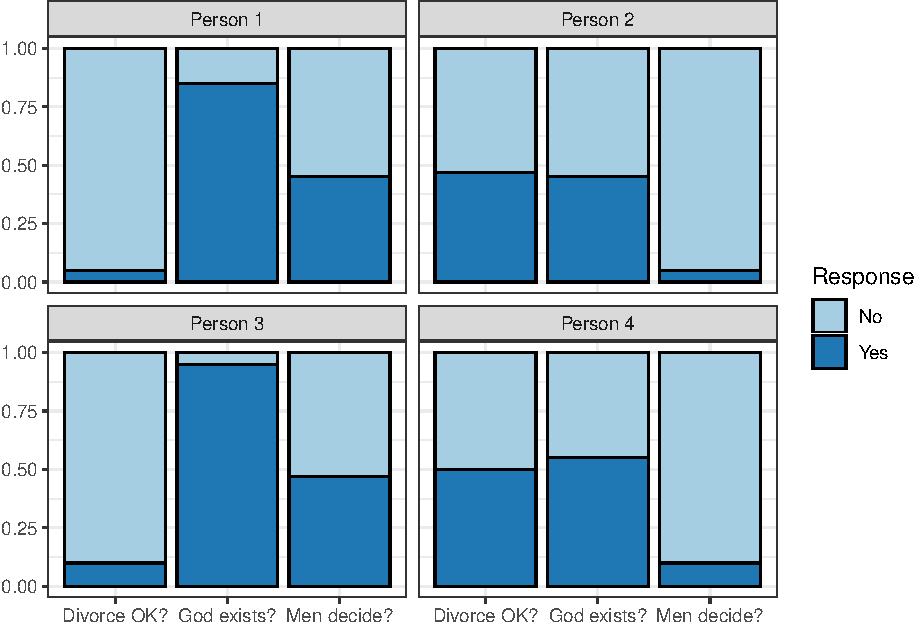
\includegraphics{rethinking_constraint_revision_files/figure-latex/sysexample-1} 

}

\caption{Hypothetical example of over-time responses for two belief systems.}\label{fig:sysexample}
\end{figure}

When we look at the distribution of responses, we would see that the two people on the left have a similar over-time distribution of response probabilities across the three questions, presumably shaped by an underlying Christian worldview that creates schematic connections between religious concepts and relationships. Because the system links marriage to the existence of a deity and eternal salvation, people with this belief system have a relatively easy time rejecting competing considerations and influences as they move across social environments, and they generate the same answer in most circumstances. A crisis of faith or actual error in filling out the survey at one time point might lead these people to say that God does not exist or that divorce is acceptable, but they present a consistent reporting of attitudes over time, regardless of the circumstances. At the same time, conflicting influences from their church and from the broader society cause them to be inconsistent on the question of gender roles as social circumstances push different considerations to the forefront of their cognition.

The two people on the right have internalized the conflicting messages present in the population about love and religion and vacillate on those two questions over time as local influences bring different considerations to the forefront of their cognition. When something triggers the prosaic model of love, such as a discussion with a friend about marital difficulties, these people say people should get divorced if they are unhappy. When something triggers the romantic model of love, such as recently watching a romantic movie, they oppose divorce. But because they lack the connection of marriage to traditional conceptions of gender roles, they have a relatively straightforward time giving the same answer to that question over time.

The key point here is that the lack of constraint on questions in each system is still a reflection of culturally patterned cognition. If we could get into the heads of the people on the right, we would see similar schematic connections from love to prosaic and romantic notions, but maybe not the religious notions of love that we would observe in the heads of the people on the left. We could trace this structure to exposure to cultural artifacts, such as movies, books, and music, and observations of how people behave in communities.

In this framework, a shared belief system is observable if we see groups of people who share probabilities of answering questions in particular ways over time and across a variety of (reasonable) social circumstances. The obvious challenge of this definition is that we do not frequently observe people's responses to the same question repeatedly over time. And if we use beliefs over time to deduce belief systems, we have nothing on which to test whether these assumptions are true. Fortunately, a method for detecting such cultural systems in cross-sectional data exists and has been used in sociological studies of attitude structuring before (Bonikowski and DiMaggio 2016; DiMaggio et al. 2018).

\hypertarget{latent-class-analysis-and-belief-systems}{%
\subsection{Latent Class Analysis and Belief Systems}\label{latent-class-analysis-and-belief-systems}}

Latent Class Analysis is a data-reduction method that seeks to group people into unobserved categories where, within these categories, the probability of giving a particular response to a question is independent from the probability of giving responses to other questions (GOODMAN 1974; Lazarsfeld and Henry 1968; McCutcheon 1987). This fundamental assumption, the conditional independence assumption, posits that once the latent class is identified, each person's response on a particular question is an independent draw from the probabilities of the different responses observed within that group.

This statistical model aligns closely with the theoretical model outlined above. LCA allows for the presence of competing sets of these cognitive structures in the population, reflected in the different latent classes. In contrast to other methods, LCA frees people to give a range of responses over time to remain in the same ``system.'' And it allows beliefs to be constrained to different degrees in different systems. In cultural sociology, LCA has been used to deduce belief systems about religion and science from survey responses in the General Social Survey (DiMaggio et al. 2018) and to deduce varieties of popular nationalism, also using the GSS (Bonikowski and DiMaggio 2016). However, these works do not make the strong assumptions about underlying cognition made here or, importantly, test these assumptions over time.

If, as the preceding discussion argues, a cultural belief system is a shared set of considerations and the connections between them that probabilistically produce certain responses over time across a range of questions, LCA should be able to detect these systems in a single wave of data. Assuming that belief systems do not undergo major revisions over time, the features of these systems observed at one time point should predict the behavior of attitudes over time.

\hypertarget{culture-and-social-structures}{%
\section{Culture and Social Structures}\label{culture-and-social-structures}}

To this point, I have assumed that cultural cognitive structures operate independently from other considerations in forming beliefs over time. This is obviously not true. Attitudes reflect a dynamic interplay between cultural-cognitive structures, social structures, and the physical environment (DiMaggio 1997; Lizardo and Strand 2010; Martin 2010; Goldberg and Stein 2018). And adjudicating the relative influence of these processes is difficult because people's cultural beliefs and preferences appear to shape their social networks and their organizational participation (Lizardo 2006; Lewis and Kaufman 2018; Vaisey and Lizardo 2010).

If differences in cognitive structures exist, they have to come from somewhere, but sociological theories disagree on how much social structure matters at different points in the life course. Some approaches suggest that most cognitive structuring occurs when people are young (Bourdieu 1990). This might be because of biological processes that make early experiences more formative for cognition, it might be because early experiences shape people's movement into subsequent social environments, or it might be because schematized cognition helps filter out compting considerations over time. Either way, this line of reasoning suggests that constrained beliefs will likely be unaffected by changing influences as people move across social structures.

Other approaches suggest cognitive structures are less durable and that social structures reshape cultural belief systems over the life course. As people move into new social environments, they get exposed to new considerations that rework their underlying cognition. Cognitive authorities, leaders endowed with the social responsibility for shaping beliefs, provide clear guidelines for which attitudes go together, and organizational hierarchies make certain belief structures appear impossible (Martin 2002). Affect-laden social interactions can make holding some attitudes feel uncomfortable, leading people to change their attitudes and producing constrained attitudes within communities (DellaPosta, Shi, and Macy 2015; Rawlings 2020). These approaches would ascribe little durability to the cognitive structures that people form and lodge a lot more explanatory power in the social environments in which people find themselves (Martin 2010).

Rethinking the hypothetical example above, it is plausible that all four people share similar underlying cognitive structures and what varies between the two pairs is their social circumstances, which shape which considerations get called up. However, if durable cognition played no role in attitude stability over time, we would expect to observe durable changes in attitudes as people move across social settings. But we tend to find the opposite, that people's dispositions are often more durable than these changing circumstances would imply (Alwin and Krosnick 1991; Kiley and Vaisey 2020; Sears and Funk 1999). This suggests that some form of durable cognitive structuring does play a role in attitude stability.

\hypertarget{hypotheses}{%
\section{Hypotheses}\label{hypotheses}}

The preceding discussion suggests a set of hypotheses about the behavior of attitudes over time. The first three hypotheses are methodological, revolving around the ability of LCA at one time point to identify belief systems that predict attitude behavior over time. The second set of hypotheses pertain to the relative role of cognitive structures in shaping attitude behavior compared to structural influences such as social networks and organizational participation.

\hypertarget{latent-class-analysis-as-a-measure-of-belief-systems}{%
\subsection{Latent Class Analysis as a Measure of Belief Systems}\label{latent-class-analysis-as-a-measure-of-belief-systems}}

The central assertion of the methodological argument is that Latent Class Analysis, using data across people at a single time point, should be able to deduce belief systems that predict within-person attitude behavior over time. As constraints -- restrictions of movement of beliefs over time -- are taken to be the central signature of a belief system (Martin 2002), I focus on those first. Specifically, the constraints on attitudes identified within a latent class at one time should predict the degree to which people change their attitudes over time. This produces the first two hypotheses:

\emph{Hypothesis 1: Within cultural belief systems, beliefs that are more constrained will demonstrate less change over time than less constrained beliefs.}

\emph{Hypothesis 2: Across cultural belief systems, the same belief will show less movement over time if it is in a belief system that constrains it more.}

The theoretical model outlined above makes a stronger prediction. It says that the belief system at time 1 should not only predict the degree to which attitudes in any particular system will change, but the probabilities that people in these belief systems will give certain responses, assuming changing social circumstances do not severely disrupt belief systems (a point I discuss below). If the theoretical model is correct, responses at any time should be conceptualized as independent draws from the distribution deduced at time 1. These probabilities are shaped by broad cultural forces that influence people's considerations, but which specific response a person gives at any wave will be shaped by (random) local influences. While it will be hard to predict what any particular person will say in each wave, especially if we are looking at an unconstrained belied, assuming these draws are independent can give us strong predictions for the overall count of observed patterns over time. This produces the third hypothesis:

\emph{Hypothesis 3: Over time, the aggregate response patterns of the sample should reflect independent draws from the deduced belief systems.}

\hypertarget{adjudicating-culture-and-structure}{%
\subsection{Adjudicating Culture and Structure}\label{adjudicating-culture-and-structure}}

The preceding hypotheses assume either that social circumstances are invariant or that changing social circumstances do not significantly affect people's belief systems. I test this assumption and, in doing so, compare the relative influence of social structures and cultural belief structures on attitudes over time.

If people have durable schematic thinking, then they should be less susceptible to the influence of alternative considerations that come from changing social environments (Hunzaker 2016). This might in part be because they select into social settings, but it should principally be because these schematic structures influence how they process new information.

The most prominent alternative model is that socially patterned collections of attitudes are largely a product of people being located in similar social structures, and that cultural background, shaping ongoing cognition through durable cognitive structures, is largely irrelevant. Under this hypothesis, the reason people exhibit similar sets of attitudes is not because they have similar cultural belief systems shaping their attitude responses over time, but because they exist in similar social environments that produce similar independent attitudes. As people move across social environments, they hear different sets of considerations that reshape their consideration sets and the attitudes they report in surveys. If this is the case, measures of social structure at the time of the survey should outperform measures of the the cultural structuring of their belief systems in the past in explaining current beliefs.

As noted previously, attitude structuring is undoubtedly an interaction between cultural schemas and social structures (DiMaggio 1997; Martin 2010; Lizardo and Strand 2010). But given a lack of evidence for durable change in attitudes over time and the fact that we observe substantially less durable change in attitudes than changing social circumstances would predict (Kiley and Vaisey 2020), I expect that belief systems play a much larger role in shaping people's attitudes over time than this structural reasoning suggests. This leads to my final hypothesis:

\emph{Hypothesis 4: Belief systems will better predict people's attitude reports over time than models that account changing social circumstances.}

\hypertarget{data-and-measures}{%
\section{Data and Measures}\label{data-and-measures}}

Testing the propositions outlined above requires data on the same beliefs and relevant social structures measured over time. The National Study of Youth and Religion meets these criteria. Below I outline the data set and measures used to test the hypotheses outlined above.

\hypertarget{the-national-study-of-youth-and-religion}{%
\subsection{The National Study of Youth and Religion}\label{the-national-study-of-youth-and-religion}}

The National Study of Youth and Religion is a four-wave panel survey of adolescents that began in 2002 when respondents were between the ages of 13 and 17 and surveyed them every three or four years for four waves (Smith 2005). The survey began with a sample of 3,370 adolescents and is designed to be a probabilistic sample of adolescents in the United States at the time the survey started in 2002. The same respondents were asked to complete subsequent waves with response rates varying over time: 2,604 at wave 2 (72 percent); 2,182 at wave 3 (65 percent); and 2,144 at wave 4 (64 percent). In wave 2, respondents were between ages 16 and 20, in wave 3 respondents were between ages 17 and 24, and in wave 4 respondents were between ages 20 and 32.

The age range of the NSYR is important to the theoretical argument outlined above as it pertains to the structuring of cognition and the movement across organizational and social contexts. Adolescence and early adulthood, the periods covered in the NSYR, are assumed to be particularly formative for cultural beliefs (Kiley and Vaisey 2020; Ghitza, Gelman, and Auerbach, n.d.; Bartels and Jackman 2014). At the same time, these periods also represent a significant time of transition for young people in the United States as they move out of their parents' homes and into college and the workforce, begin to form long-term romantic attachments, and generally transition from adolescence to adulthood. There is likely more movement across social contexts at this period than most other periods in the life course. As such, this provides a good window in which to test the competing influences of cultural belief structures, organizational settings, and social change.

My analysis focuses principally on Waves 2 through 4 of the NSYR.\footnote{Many of the attitude measures used in this analysis were not added to the survey until wave 2. Focusing on attitudes present in all four waves severely curtails the number of beliefs that can be explored.} Because I only draw a few background variables from the first wave of the NSYR, and because time matters significantly in the testing of the theoretical model outlined above, for clarity I will refer to waves 2, 3, and 4 of the NSYR as times 1, 2, and 3 for the rest of this paper.

Deducing belief systems at time 1 requires people to have responses on all belief measures and covariates. Because the relationships among beliefs are a central question of this analysis, any missing data imputation strategy might bias the deduction of classes in unforeseen ways. To measure belief systems, I only use people who are observed on all covariates and beliefs at time 1, leaving a sample of 2,521 respondents. Testing hypotheses 1 and 2 requires people to have beliefs observed at all three time points, but it does not necessarily require covariates in later waves, and the test does not require people to be observed on all beliefs. As a result I use data on people whose classes are deduced at time 1 and who were observed on any beliefs at times 2 and 3. The sample size for each question varies between 1,668 (divorceok) and 1,699 (demons).

Testing hypothesis 3 and 4 requires comparable social structure and belief variables over time. Because some key social structural questions were dropped at time 3 (specifically questions about social networks), I focus on change between times 1 and 2. Again, it is not necessary that respondents report all beliefs at time 2, but respondents must have full beliefs at time 1 and full covariates at times 1 and 2. The analytical samples range from 2,153 (divorceok) to 2,175 (demons).

\hypertarget{measures}{%
\subsection{Measures}\label{measures}}

\hypertarget{beliefs}{%
\subsubsection{Beliefs}\label{beliefs}}

In times 1 through 3, NSYR respondents were asked a set of questions about their religious, moral, and family-structure beliefs. Seven questions ask about religious beliefs, four ask about morality and the role of religion in daily life, and six ask about gender relations and family structures.\footnote{An obvious omission from this list of questions is the one Vaisey (2009) uses to predict adolescent behavior and social networks over time, which he argues represents people's ``moral typology.'' Because of a coding error, responses to that question were lost for almost all respondents at Wave 3 of the NSYR, making it hard to compare across waves.} These questions are reported on either a three-point scales of ``yes,'' ``maybe,'' and ``no,'' or five-point scales of ``strongly agree,'' ``agree,'' ``undecided/don't know,''\footnote{Responses of ``don't know'' were not provided in the survey for questions asked on the five point scales, but if respondents gave them, they were coded as such. As such, they are relatively rare. When responses to questions that include a ``maybe'' option are coded as ``don't know,'' I recode these responses to the ``maybe'' response.} ``disagree,'' ``strongly disagree.'' These variables are summarized in Table \ref{tab:beliefs}.

\begin{table}
\scriptsize
\begin{center}
\begin{tabular}{l l c c c c c c c}
\hline
\\
Religion & Do you believe... & Time & 1. Yes &   & 3. Maybe &   & 5. No & N. Obs.\\
\hline
 aftrlife &  ...that there is life after death? & 1 & 1188 &  & 1078 &  & 255 & 2521\\
 &  & 2 & 1075 &  & 886 &  & 207 & 2168\\
 &  & 3 & 862 &  & 640 &  & 197 & 1699\\
 angels &  ...in the existence of angels? & 1 & 1403 &  & 866 &  & 252 & 2521\\
 &  & 2 & 1187 &  & 734 &  & 254 & 2175\\
 &  & 3 & 910 &  & 488 &  & 298 & 1696\\
 astrolgy  & ...in astrology, that stars and  & 1 & 301 &  & 579 &  & 1641 & 2521\\
 & planets affect people's lives? & 2 & 225 &  & 451 &  & 1498 & 2174\\
 &  & 3 & 140 &  & 521 &  & 1036 & 1697\\
 demons  & ...in the existence of demons or  & 1 & 1118 &  & 834 &  & 569 & 2521\\
 & evil spirits? & 2 & 980 &  & 639 &  & 556 & 2175\\
 & & 3 & 754 &  & 575 &  & 370 & 1699\\
 god & ...in God, or not, or are you unsure? & 1 & 1950 &  & 448 &  & 123 & 2521\\
 & & 2 & 1662 &  & 378 &  & 134 & 2174\\
 &  & 3 & 1206 &  & 285 &  & 204 & 1695\\
 godworld & ...God created the world? & 1 & 1731 &  & 125 &  & 665 & 2521\\
 &  & 2 & 1414 &  & 119 &  & 630 & 2163\\
 &  & 3 & 706 &  & 582 &  & 408 & 1696\\
 heaven & ...in heaven as a place where some  & 1 & 2121 &  & 35 &  & 365 & 2521\\
 & people go after death? & 2 & 1778 &  & 18 &  & 376 & 2172\\
 & & 3 & 1106 &  & 311 &  & 281 & 1698\\
 miracles & ...in the possibility of divine miracles? & 1 & 1531 &  & 696 &  & 294 & 2521\\
 & & 2 & 1317 &  & 557 &  & 300 & 2174\\
 & & 3 & 922 &  & 505 &  & 272 & 1699\\
 reincar & ...in reincartion, that people  & 1 & 436 &  & 766 &  & 1319 & 2521\\
 & have lived previous lives? & 2 & 312 &  & 655 &  & 1206 & 2173\\
 &  & 3 & 213 &  & 701 &  & 779 & 1693\\
\hline
 &  &  & 1. Strongly &  & 3. Unsure/ &  & 5. Strongly & \\
Morality & & Time & Agree & 2. Agree & DK & 4. Disagree & Disagree & N. Obs.\\
\hline
 brkmoral & It is sometimes okay to break moral  & 1 & 28 & 352 & 7 & 1531 & 603 & 2521\\
 & rule if it works to your  & 2 & 35 & 321 & 5 & 1129 & 678 & 2168\\
 & advantage. & 3 & 19 & 111 & 97 & 873 & 593 & 1693\\
 moralchg  & The world is always changing and we   & 1 & 272 & 1272 & 19 & 702 & 256 & 2521\\
 & should adjust our views of what is  & 2 & 215 & 1130 & 17 & 610 & 195 & 2167\\
 & morally right. & 3 & 149 & 606 & 161 & 491 & 282 & 1689\\
 moralrel  & Morals are relative, there are no definite   & 1 & 221 & 1224 & 33 & 744 & 299 & 2521\\
 & rights and wrongs for everybody. & 2 & 146 & 876 & 10 & 817 & 316 & 2165\\
 & & 3 & 125 & 489 & 117 & 637 & 322 & 1690\\
 relprvte & Religion is a private matter that should   & 1 & 368 & 1076 & 13 & 829 & 235 & 2521\\
 & be kept out of public debates. & 2 & 400 & 919 & 10 & 661 & 177 & 2167\\
 &  & 3 & 433 & 574 & 139 & 381 & 162 & 1689\\
\hline
 &  &  & 1. Strongly &  & 3. Unsure/ &  & 5. Strongly & \\
Family &  & Time & Agree & 2. Agree & 3. DK & 4. Disagree & Disagree & N. Obs.\\
\hline
 divrceok  & A couple without children should    & 1 & 1755 &  & 37 &  & 729 & 2521\\
 & end their marriage if it is  & 2 & 1483 &  & 26 &  & 644 & 2153\\
 & empty and unfulfilling? & 3 & 1183 &  &  0 &  & 499 & 1682\\
 mandecid  & Most of the important decisions in the   & 1 & 68 & 380 & 6 & 1429 & 638 & 2521\\
 & life of the family should be made by  & 2 & 54 & 322 & 16 & 1101 & 674 & 2167\\
 & the man of the house. & 3 & 47 & 181 & 57 & 759 & 644 & 1688\\
 manmar & A man can have a fully satisfying life   & 1 & 403 & 1646 & 8 & 404 & 60 & 2521\\
 & without getting married. & 2 & 412 & 1392 & 8 & 287 & 71 & 2170\\
 &  & 3 & 526 & 863 & 70 & 187 & 47 & 1693\\
 unmarsex  & It is alright for two unmarried people    & 1 & 157 & 1177 & 9 & 862 & 316 & 2521\\
 & who are not in love to have sex. & 2 & 175 & 1104 & 13 & 663 & 211 & 2166\\
 & & 3 & 398 & 723 & 80 & 309 & 180 & 1690\\
 wommar & A woman can have a fully satisfying life   & 1 & 459 & 1632 & 16 & 371 & 43 & 2521\\
 & without getting married. & 2 & 485 & 1362 & 10 & 269 & 44 & 2170\\
 &  & 3 & 531 & 850 & 89 & 184 & 38 & 1692\\
 wrkngmom & A working mother can establish as warm    & 1 & 489 & 1581 & 12 & 401 & 38 & 2521\\
 & and secure a relationship with her children    & 2 & 440 & 1303 & 9 & 374 & 40 & 2166\\
 & as a mother who does not work. & 3 & 594 & 836 & 70 & 166 & 23 & 1689\\
\hline
\end{tabular}
\caption{Belief measures}
\label{table:beliefs}
\end{center}
\end{table}

These responses are treated as nominal in some models and continuous in others. To make the range of responses to each question comparable, I scale all attitude measures to five-point scales between 1 and 5 by converting questions on three point scales: ``yes'' to 1, ``maybe'' to 3, and ``no'' to 5.

\hypertarget{covariates}{%
\subsubsection{Covariates}\label{covariates}}

Given the belief domains explored here, I examine three principal sources of attitude structuring: sociodemographic backgrounds, participation in organizations, and social networks. Sociodemographic background variables include respondent gender (indicator for female), and whether at least one parent has a bachelor's degree.\footnote{These demographic variables are measured at the survey's first wave and are assumed to be invariant during the survey. Preliminary analyses found that other demographic variables, including race/ethnicity, parent's income, and whether people grew up in a two-parent household were unrelated to beliefs, net of other predictors.}

A second set of covariates is designed to tap organizational participation, which is expected to change to some extent between waves. Given the role of religious organizations in shaping attitudes explored here, I include a set of indicator variables for religious tradition (Steensland et al. 2000) and a measure of church attendance, measured on a scale from never (0) to more than once a week (6).\footnote{The NSYR includes a separate indicator for members of the Church of Jesus Christ of Latter-day Saints. The religious tradition measure places members of the Church of Jesus Christ of Latter-day Saints in the ``other'' category. I group these respondents with evangelical protestants, based on preliminary analysis of their response patterns. While there are deep theological differences between the groups, these are not reflected in the questions analyzed here, and the two groups behave similarly in terms of the beliefs measured in this analysis. The NSYR also includes a code for respondents with an indeterminate religion, separated by whether they attend services or not. I group these into a distinct category of indeterminate religious tradition. Finally, the NSYR includes separate codes for ``black Evangelical protestants'' and ``black Mainline protestants.'' I group these two categories together.} Because participation in formal education might introduce an alternative set of considerations into people's belief systems, I include a variable measuring the number of years of education a person has received above ninth grade. I also include an indicator for whether the respondent lives in the South census region to capture movement across geographic contexts. Other census regions were uncorrelated with beliefs.

Finally, to measure social network influence, I include the proportion of a respondents' friends who share that person's religious orientation, including no religious orientation for people who do not express one.\footnote{Almost all respondents at time 1 (about 94 percent) said they had five close friends, making a count of friends as an additional measure superfluous.} As a second measure of social networks, I include the highest level of closeness a respondent reported with either parent.

These covariates are measured at times 1 and 2.

\hypertarget{belief-systems}{%
\subsection{Belief Systems}\label{belief-systems}}

I use Latent Class Analysis to deduce a set of belief systems using the 19 attitude items asked at time 1. LCA attempts to assign a class to each respondent such that their responses are independent from each other within classes. The model uses the Newton-Raphson method to maximize the log-likelihood of multiple parameters under the assumption that indicators are independent conditional on class membership.

A model that predicts the observed response pattern \(y\) using a latent class variable \(X\) with \(L\) values has the following probability structure:

\[ P(Y=y) = \sum_l P(X=l)P(Y=y|X=l)\]

Because of the conditional independence assumption that \(K\) indicators are independent within each latent class \(l\), the joint probability of a given response pattern can be rewritten as the product of individual item response probabilities, and \(P(Y=y|X=l)\) can be rewritten as:

\[\prod_{k}P(Y_k = y_k | X=l) \]

LCA estimates a set of parameters that includes the relative class proportions and the probabilities of each response for each class on each question. For the purposes of the LCA, responses to the belief questions are treated as nominal.

The model also includes the covariates outlined above as predictors of class assignment. The model simultaneously estimates two conditional probabilities: the probability of response conditional on group assignment and the probability of group assignment conditional on covariates. I use the Bayesian information criterion to select the best-fitting number of classes.

\hypertarget{testing-hypotheses}{%
\subsection{Testing Hypotheses}\label{testing-hypotheses}}

\hypertarget{change-over-time}{%
\subsubsection{Change Over Time}\label{change-over-time}}

The first two hypotheses make predictions about how much attitudes should change over time as a function of the constraint within a belief system at a single point in time. Within a system, more constrained beliefs should change less over time than less constrained beliefs, and across systems, a belief should change less in a more constrained system.

I measure constraint of a particular attitude, \(j\), for members of a designated belief system, \(k\), by calculating the within-class standard deviation of responses to that question over all people, \(i\). LCA assigns each person a probability of belonging to a each class. For this analysis, I assign each person to the class with the highest probability. I then calculate the standard deviation of responses within that group, treating responses as continuous, rather than nominal as the LCA does. A group where people tend to give the same response or cluster in adjacent responses will have a low standard deviation and therefore high constraint. A group where people tend to give answers across the scale will have a high standard deviation and therefore low constraint.

\[ \sigma_{jk} = \sqrt{ \frac{\sum{(x_{ijk} - \mu_{jk})^2}}{N_k - 1}}  \]

The outcome of interest is the amount of variation people express in their attitudes over time. I measure within-person variance over time using the within-person standard deviation of responses given at times 1, 2, and 3.

\[ \sigma_{ij} = \sqrt{ \frac{\sum{(x_{ijt} - \mu_{ij})^2}}{N_{i} - 1}}  \]

I test the first and second hypothesis using a single linear regression of within-person variance on the within-class standard deviation at time 1, with fixed effects for question (\(J\)) and for person (\(I\)). This amounts to simultaneously testing whether people exhibit more variation in their less constrained beliefs over time than their more-constrained beliefs and whether a belief demonstrates more over-time variation when it is in a less constrained belief system than when it is in a more constrained belief system.

\[ \sigma_{ij} = \sigma_{jk} + I + J + \epsilon_{ij} \]

I also conduct a similar fixed-effects regression of each person's mean for each question at times 2 and 3 (\(\mu_{ij,t>1}\)) on the group mean at time 1 (\(\mu_{jk}\)) for each question at time 1. This tests whether constraints about where group members fall on average continue to constrain people over time.

\[ \mu_{ij,t>1} = \mu_{jk} + I + J + \epsilon_{ij} \]

\hypertarget{pattern-prediction}{%
\subsection{Pattern Prediction}\label{pattern-prediction}}

The remaining hypotheses posit that modeling people's responses over time as independent draws from the belief system outperforms other potential data-generating processes. To assess this proposition, I take a predictive approach (Hofman, Sharma, and Watts 2017; Salganik et al. 2020).

Hypotheses 3 and 4 focus on the observed counts of change patterns over time. To illustrate this approach, assume two belief systems that differently constrain people's views on the following question: ``Do you think that, in general, a couple without children should end their marriage if it is empty and unfulfilling, or should they stick with it even if they are not happy?'' In one belief system, people are constrained to oppose divorce quite strongly (\(Pr(yes)=.9\)). These people have many considerations against divorce, but there is a small chance that a local event could make them support it. In the second belief system, people have roughly equal considerations in favor of and opposed to divorce (\(Pr(yes)=.5\)). Which response they give at a particular wave will be affected by the balance of considerations on their mind at any time.

If responses over time are independent draws from this distribution, then if we asked people the question two times, people in the first group should say ``yes'' in both waves about 81 percent of the time (\(.9 * .9 = .81\)). People in the second group should say ``yes'' in both waves about 25 percent of the time (\(.5 * .5 = .25\)). We can calculate the probability of each of the four possible two-wave response patterns, presented below:

\begin{longtable}[]{@{}lcc@{}}
\toprule
Pattern & \(Pr(yes)=.9\) & \(Pr(yes)=.5\)\tabularnewline
\midrule
\endhead
Yes -\textgreater{} Yes & .81 & .25\tabularnewline
Yes -\textgreater{} No & .09 & .25\tabularnewline
No -\textgreater{} Yes & .09 & .25\tabularnewline
No -\textgreater{} No & .01 & .25\tabularnewline
\bottomrule
\end{longtable}

A key assumption of the belief systems model is that predicting any person's response at any particular time will be difficult, especially if it is deduced that beliefs are relatively unconstrained in a particular system, such as in the rightmost column. But since it assumes local influences are statistically random, the theoretical model can generate strong predictions of counts of response patterns in the aggregate. I can use the distribution of these two belief systems in the population, as well as the distribution of responses observed at time 1, to generate a range of plausible predictions for the count of each pattern.

Predicting response patterns in the latent class model requires two steps: sampling class identification and sampling responses. The LCA model assigns each observation a probability of belonging to each class based on their covariate profile. I sample class assignment from these probabilities. Then, using these class assignments, I sample responses from the probabilities assigned to members of that class. I count the number of people who demonstrate each response patterns (``Agree'' at time 1 to ``Disagree'' at time 2) and compare that to the observed count of response patterns. While the theoretical framework makes within-class predictions, because people are probabilistically assigned to different classes, and to make comparisons to other theoretical processes, I aggregate counts of response patterns at the question level.

To measure the predictive accuracy of a model for each question, \(j\), I square the difference between the expected number of response patterns generated by the model for all combinations of responses at time 1 and time 2, \(E_{j}(t_1, t_2)\), and the observed number of cases that had that response pattern, \(O_{j}(t_1, t_2)\), penalizing larger deviations. I then sum across all potential patterns and take the square root of this value to get a measure of predictive accuracy.

\[ \lambda_j =  \sqrt{\sum_{t_1}\sum_{t_2}(E_j(t_1, t_2) - O_j(t_1, t_2))^2} \]

Because both class assignment and response probabilities reflect sources of uncertainty, I iterate this process 10,000 times to generate a distribution of accuracy that reflects the probabilities of class assignment and response probabilities.

This range of numbers provides a quantification of how good the model predicts response patterns, with 0 being a perfect prediction of the count of response patterns. But this range is meaningless on its own, since there is no clear alternative expectation for how many counts we might observe. It is unlikely that any model would perfectly predict responses over time. But I can compare this theoretical process to other theoretical models. To generate an plausible upper-bound of prediction, I sample from the marginal distribution at wave 3 for each respondent.

The first theoretically grounded alternative to the belief system model suggests beliefs are independent from each other. In this framework, belief in the existence of God is independent from considerations of divorce, and there is no underlying belief system that influences both. Under this model, people have more or less idiosyncratic belief systems (or sets of considerations) as a function of their social experiences. People would receive separate influences on each belief from their social environments -- churches, schools, families, friends, etc. -- and these would shape their responses at each wave.

To estimate these idiosyncratic resposes, I conduct a multinomial logistic regression for each individual attitude at time 1 using the same set of covariates included in the latent class analysis.\footnote{This approach assumes that each person's response at each wave is a draw from a multinomial distribution. An alternative is to assume that each person's response is a latent variable observed with error. This would model the outcome not as a set of independent categories (multinomial logit/probit), but as manifestation of a latent variable (ordinal logit/probit). In practice, the multinomial logit is a less constrained version of the ordinal logit model. If attitudes do reflect an underlying latent construct, the multinomial logit will reflect this structure, but the reverse is not true. Since I am not principally concerned with model parsimony, but rather on adjudicating theoretical processes, I use the multinomial logit model.} This produces a set of individual-specific probabilities of giving each response to a question. I then use those probabilities to simulate responses over time and similarly quantify predictive accuracy.

Model comparisons typically penalize models for complexity, as complexity leads to greater predictive accuracy within a sample. The latent class model, while complex, is simpler than estimating separate models for each belief. If the latent class model makes better predictions, there is no reason to prefer estimating separate probabilities for each response on the grounds of parsimony. There are obvious ways to simplify both models by removing parameters that do not aid in prediction, or by treating responses as ordinal rather than multinomial. However, the goal of using the same predictors and same outcome scale is to design two models that reflect two similar but distinct theoretical processes: one where beliefs influence and constrain each other, and one where they do not.

\hypertarget{changing-circumstances}{%
\subsection{Changing Circumstances}\label{changing-circumstances}}

Hypothesis testing to this point has been oriented toward establishing LCA as a good methodological fit for the theoretical concept of a belief system and the predictions it makes over time. If that is established, then I can use the deduced belief systems to compare the relative influence of the belief system with social structural changes that might produce changes in beliefs over time.

Both the LCA model and the idiosyncratic beliefs model outlined above assume that belief systems are shaped early in life and endure, but Hypothesis 4 suggests that changing social circumstances will reshape beliefs over time. To test the influence of organizational and social network change, I use the coefficients derived from the latent class and multinomial logit model at time 1 to predict class assignment and responses at time 2 using social structural and social network variables observed at time 2. If changing circumstances -- increased church attendance or a more diverse friend group, for example -- have the effect of producing changes in attitudes, then using information about social change between waves will produce better estimates of the patterns of change over time.

This approach makes a rather strong assumption that the coefficients estimated at time 1 hold at time 2, but that is what is inherent in the strong structural argument. Under these approaches, beliefs at time t are a reflection of structures at time t. If coefficients derived at time 1 are a bad predictor of beliefs at time 2, it suggests that different influences matter at each time point.

To ensure comparability across prediction models, each prediction model uses all people with full beliefs and covariates at time 1 to generate coefficients (2,521 respondents), and people with beliefs at time 1 and all observed covariates at times 1 and 2. A handful of people with covariates at time 2 failed to answer some of the belief questions. They are evaluated on the questions they did respond to.

\hypertarget{results}{%
\section{Results}\label{results}}

The results proceed in three parts. First, I deduce and explain the belief systems identified through LCA. Second, I test the proposition that the constraints implicit in each belief system are good predictors of over-time change. Third, I adjudicate the competing influences of the belief system and social structures in predicting responses over time.

\hypertarget{belief-systems-1}{%
\subsection{Belief Systems}\label{belief-systems-1}}

Based on goodness of fit measures and substantive interpretation, I selected and present a five-class model to summarize the belief systems across the three domains outlined above. Figure \ref{fig:beliefsystems} presents the expected probability of each response option for all 19 questions for all of the classes. Table \ref{tab:classcovs} summarizes the distribution of covariates across classes. I briefly summarize each belief system, giving a substantive interpretation based on response probabilities and covariates, as well as their implications for expected over-time change.

\begin{figure}

{\centering 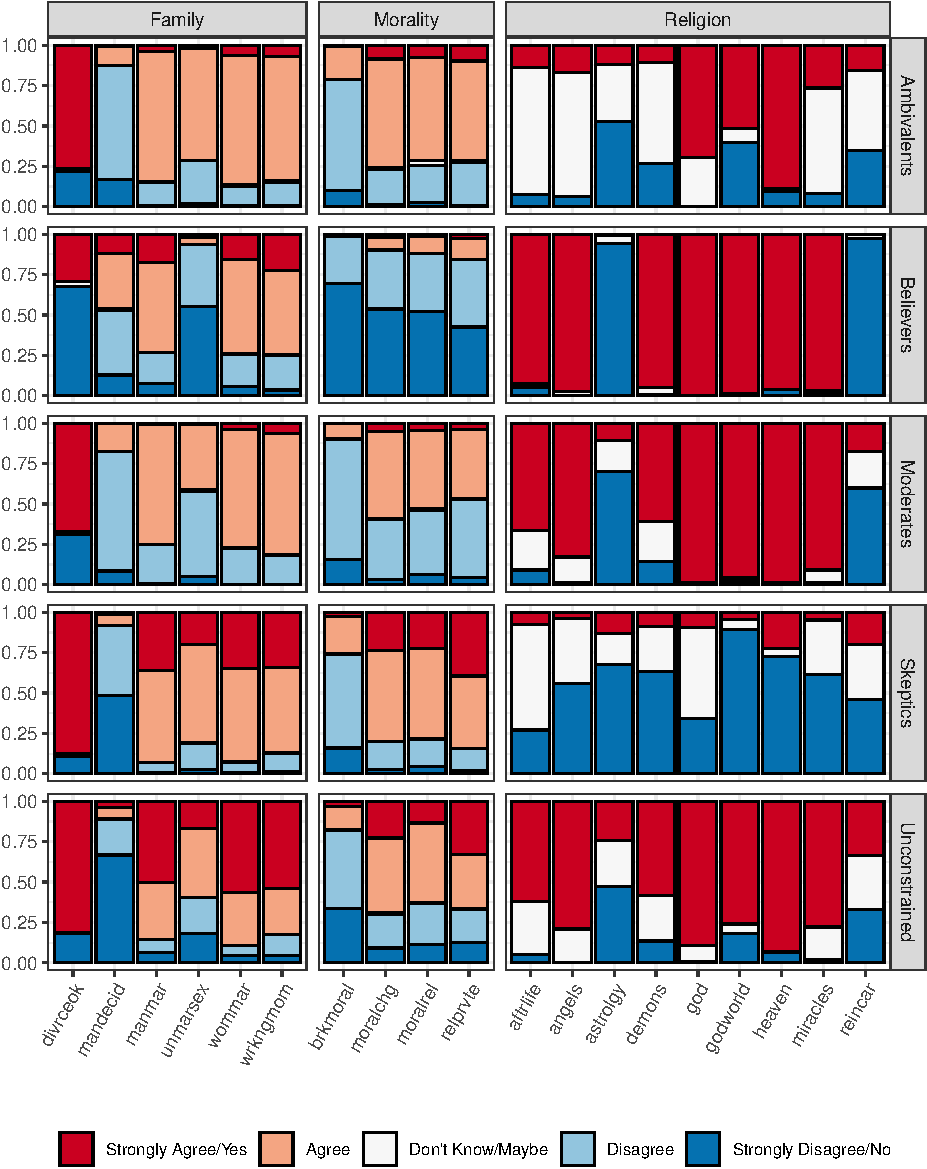
\includegraphics{rethinking_constraint_revision_files/figure-latex/beliefsystems-1} 

}

\caption{Religious, Moral, and Family Beliefs by Class}\label{fig:beliefsystems}
\end{figure}

\begin{table}
\small
\begin{center}
\begin{tabular}{l c c c c c}
\hline
 &  &  & True  &  & \\
 & Skeptics & Ambivalents & Believers & Moderates & Unconstrained\\
\hline
Class prevalence & 0.14 & 0.27 & 0.13 & 0.32 & 0.15\\
\\
Black Protestant & 0.04 & 0.24 & 0.07 & 0.49 & 0.16\\
Catholic & 0.05 & 0.45 & 0.02 & 0.28 & 0.19\\
Indeterminate Religion & 0.06 & 0.23 & 0.10 & 0.45 & 0.16\\
Evangelical Protestant/LDS & 0.01 & 0.11 & 0.34 & 0.44 & 0.10\\
Jewish & 0.46 & 0.41 & 0.01 & 0.02 & 0.10\\
Mainline Protestant & 0.07 & 0.28 & 0.10 & 0.38 & 0.17\\
No Affiliation & 0.48 & 0.34 & 0.00 & 0.06 & 0.12\\
Other & 0.30 & 0.15 & 0.15 & 0.22 & 0.18\\
\\
Female & 0.11 & 0.22 & 0.14 & 0.34 & 0.19\\
Male & 0.16 & 0.32 & 0.12 & 0.30 & 0.10\\
\\
South & 0.09 & 0.20 & 0.16 & 0.40 & 0.15\\
Not South & 0.17 & 0.32 & 0.11 & 0.27 & 0.13\\
\\
Parents have B.A. & 0.19 & 0.26 & 0.17 & 0.26 & 0.12\\
Parents do not have B.A. & 0.10 & 0.27 & 0.10 & 0.37 & 0.16\\
\\
Mean age & 17.65 & 17.66 & 17.76 & 17.67 & 17.85\\
Mean service attendance (0-6) & 0.53 & 1.74 & 5.12 & 3.26 & 2.10\\
Years of education & 11.53 & 11.29 & 11.65 & 11.41 & 11.56\\
Parental closeness (1-6) & 4.80 & 4.99 & 5.26 & 5.09 & 5.22\\
Prop. friends share belief & 0.48 & 0.54 & 0.79 & 0.70 & 0.63\\
\hline
\end{tabular}
\caption{Covariates of class assignments}
\label{table:classcovs}
\end{center}
\end{table}

\emph{Believers:} The first group, about 13 percent of survey respondents, has strongly constrained religious and moral beliefs. Almost everybody in this class expresses a belief in the major tenets of Christian theology, and they reject non-Christian beliefs (reincarnation and astrology). They strongly contrast with other classes in being much more likely to say they disagree and strongly disagree with moral relativism (moralchg; moralrel) and the notion that religion is a private matter (relprvte). They are also strongly constrained to believe that sex before marriage is wrong. Identification as an Evangelical Protestant/LDS is a strong predictor of being in this class, and members of this group attend religious services substantially more often than members of other classes.

A key feature of this class is that they are less constrained in their beliefs about family and gender than many of the other classes. This lack of constraint arises because their belief space is broader than that of other classes; their belief system presents them considerations that are at odds with the prevailing culture. While most classes tend to think that men and women can live a ``fully satisfying life without getting married,'' members of this group appear to have considerations that push them to disagree. Similarly, while most other groups are constrained to the ``disagree'' side of the scale on whether ``Most of the important decisions in the life of the family should be made by the man of the house,'' members of this group occasionally agree or strongly agree. They are also the group most likely to say that sex before marriage is not acceptable.

Under the belief system framework outlined above, I expect members of this group to be highly unlikely to make changes in their beliefs about religious phenomena, both relative to their other beliefs and relative to other groups. They will also be less likely to change their views of morality than members of other groups. At the same time, because they have conflicting considerations about family structures, they should be more likely to change those beliefs -- both more likely to change them than other groups and more likely to change them than other beliefs.

\emph{Skeptics:} The second class, about 14 percent of respondents, is characterized by a rejection or questioning of religious beliefs. They also reject or question astrology and reincarnation. In fact, they look more similar to Believers on these two issues than other classes do. They are the most constrained to the ``relative'' side of the moral relativism-moral absolutism scales. In terms of covariates, they tend not to identify with a religious denomination or attend religious services. However, people who identify as Jewish cluster in this group.

This group is also quite constrained on some religious beliefs, some family structure questions, and views on morality, though in the opposite direction from Believers. They should change little on these beliefs over time. They are the least constrained on the question of god's existence, about equally split between saying ``no'' and ``maybe.'' I expect members of this group to vacillate on this question.

\emph{Moderates:} This group, the largest in the sample with about 32 percent of respondents, closely resembles the Believers in their responses to questions about religious beliefs, but their constrained religious beliefs do not appear to spill over into other domains. Members of this group appear torn between their religious commitments and the culture of contemporary American society, or at least have not taken the time to reconcile these contradictions, producing relatively high levels of ambivalence on issues of family structure and morality, rarely giving ``strong'' responses to either. This is the largest class in the data set, drawing members from all religious groups, principally people who do attend religious services but do not attend them frequently.

\emph{Ambivalent:} The third group, about 27 percent of respondents, is characterized by a high degree of uncertainty on religious and moral beliefs. They are the most likely to say ``maybe'' in response to questions about the existence of angels, demons, and God, as well as the non-Christian belief questions such as astrology and reincarnation. These respondents tend to be Catholic or unaffiliated with a religious tradition and infrequent service attenders. Members of this group are the least likely to give strong opinions on questions of morality and family structures.

\emph{Unconstrained:} The final group, about 15 percent of the sample, demonstrates little constraint across the board. While it is tempting to interpret this group as displaying idiosyncratic belief systems, the theoretical model suggests that these people have internalized a broad range of considerations that make them highly subject to local influences. As a result, they should vacillate over time on these questions, especially questions about morality, where they give both moderate and strong opinions on both sides of the issue.

Contrasting this Unconstrained group with the Ambivalent group helps draw out the theoretical implications of the belief system model. Members of the Ambivalent group explicitly pick scale midpoints, while members of the unconstrained group range widely. This suggests the former demonstrate a higher level of constraint in their cognition, recognizing their conflicting considerations and averaging them. Members of the latter group appear not to recognize these conflicts and appear to be more subject to the whims of temporary influences. Where a member of the Ambivalent group might say that morality is a complicated mix of relativism and absolutism, members of the Unconstrained group might strongly agree that morality is relative at one moment and strongly disagree at another.

While I call these five groups ``belief systems,'' it is not necessary that members of these groups see these domains or beliefs as connected. It could be the case that the group I have deemed Moderates do not see connections between family life, morality, and religious behavior. These groups should be conceptualized as socially patterned sets of influences -- schooling, parent's education, social networks, and religious participation -- that shape the range of considerations members hold.

With the exception of the Unconstrained group, most of these groups present some level of constraint in a portion of the belief space. Both Believers and Skeptics are constrained in their religious, moral, and (most) family beliefs, though in different ways. Moderates have constraints on religious beleifs. Ambivalents are somewhat uniquely constrained to the middle of scales.

\hypertarget{change-over-time-1}{%
\subsection{Change Over Time}\label{change-over-time-1}}

Figure \ref{fig:standardeviation} plots the average within-question, within-class standard deviation at time 1 against the average within-question, within-person standard deviation over time. If within-group constraint of a particular question is a good proxy for within-person considerations, there should be a positive correlation between these two measures.

\begin{figure}

{\centering 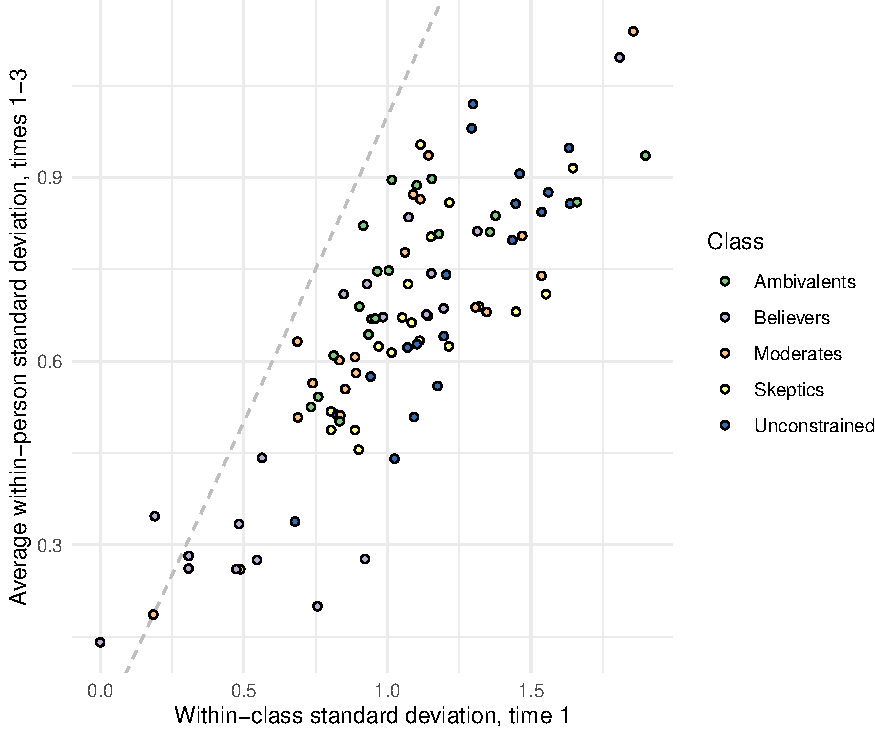
\includegraphics{rethinking_constraint_revision_files/figure-latex/standardeviation-1} 

}

\caption{Scatterplot of Within-group Standard Deviation at Time 1 against Average Within-Person Standard Deviation, Times 1-3 }\label{fig:standardeviation}
\end{figure}

There is an incredibly strong relationship between the amount that a particular question varies within a group at time 1 and the average within-person standard deviation that members of the group demonstrate over time (\(\rho = 0.829\)). This relationship holds across questions within groups (lowest correlation is 0.650 for Skeptics; highest correlation is 0.876 for the Believers) and within questions across groups, ranging from 0.449 for belief in the afterlife to 0.969 for whether divorce is acceptable.

The diagonal line in Figure \ref{fig:standardeviation} represents a 1:1 prediction of within-group variance at time 1 and average within-person variance over time, which is what we would expect if the variation observed in the classes was a perfect prediction of people's internal belief systems. Points generally fall below the line, suggesting that people are more constrained than their belief systems would suggest. This is not surprising, as idiosyncratic cognitive and social forces likely further constrain beliefs over time. But many attitudes fall very close to this line, suggesting a good fit with the theoretical model. A similar comparison of within-group means at time 1 to the groups' average means at times 2 and 3 also produces a very strong positive correlation, close to the 1:1 prediction line (\(\rho = 0.978\)).

To test hypotheses 1 and 2, I estimate a regression of within-person change between times 2 and 3 on within-group variance at time 2 with fixed effects for question and person. Table \ref{tab:coefficients} presents the results of that regression. I also present a regression of the group mean at time 1 on within-person means for times 2 and 3 to examine whether people are, in general, constrained to the same portion of the belief space.

\begin{table}
\begin{center}
\begin{tabular}{l c c}
\hline
 & Model 1 & Model 2 \\
\hline
grp\_sd    & $0.55^{***}$ &              \\
           & $(0.01)$     &              \\
grp\_mean  &              & $0.80^{***}$ \\
           &              & $(0.01)$     \\
\hline
Num. obs.  & $32102$      & $32102$      \\
\hline
\multicolumn{3}{l}{\scriptsize{$^{***}p<0.001$; $^{**}p<0.01$; $^{*}p<0.05$}}
\end{tabular}
\caption{Fixed effects linear regression of within-person, within-question standard deviation, times 1-3, on within-question latent class standard deviations, time 1.}
\label{table:femodels}
\end{center}
\end{table}

As expected, Table \ref{table:femodels} shows a strong positive association between within-group variance at time 1 and within-person change over time. In other words, consistent with Hypothesis 1, people are more likely to change attitudes that are less constrained in their group at time 1. And consistent with Hypothesis 2, within questions, groups that are less constrained exhibit more change their answers over time. The second columns show that people are, on average, highly constrained to parts of the belief space indicated by their class at wave 1, even if they sometimes have wide variance within that.

\hypertarget{predicting-response-patterns}{%
\subsection{Predicting Response Patterns}\label{predicting-response-patterns}}

Hypothesis 3 predicts responses people give over time will reflect a multinomial draw from the probabilities derived from the belief system at time 1. Figures \ref{fig:predictionerrorrel} and \ref{fig:predictionerrornotrel} compare the accuracy of predicted counts of response patterns with predictions generated using the marginal distribution at wave 3 and predictions generated from the multinomial logit model reflecting independent belief formation, for the religion variables and non-religion variables, respectively. While an overall count of accuracy across all beliefs can be estimated, beliefs are plotted separately to highlight where the belief system improves predictive accuracy and where it does not. Because the marginal distributions shape the total amount of deviance possible, each plot has a different y-axis, though all begin at 0.

\begin{figure}

{\centering 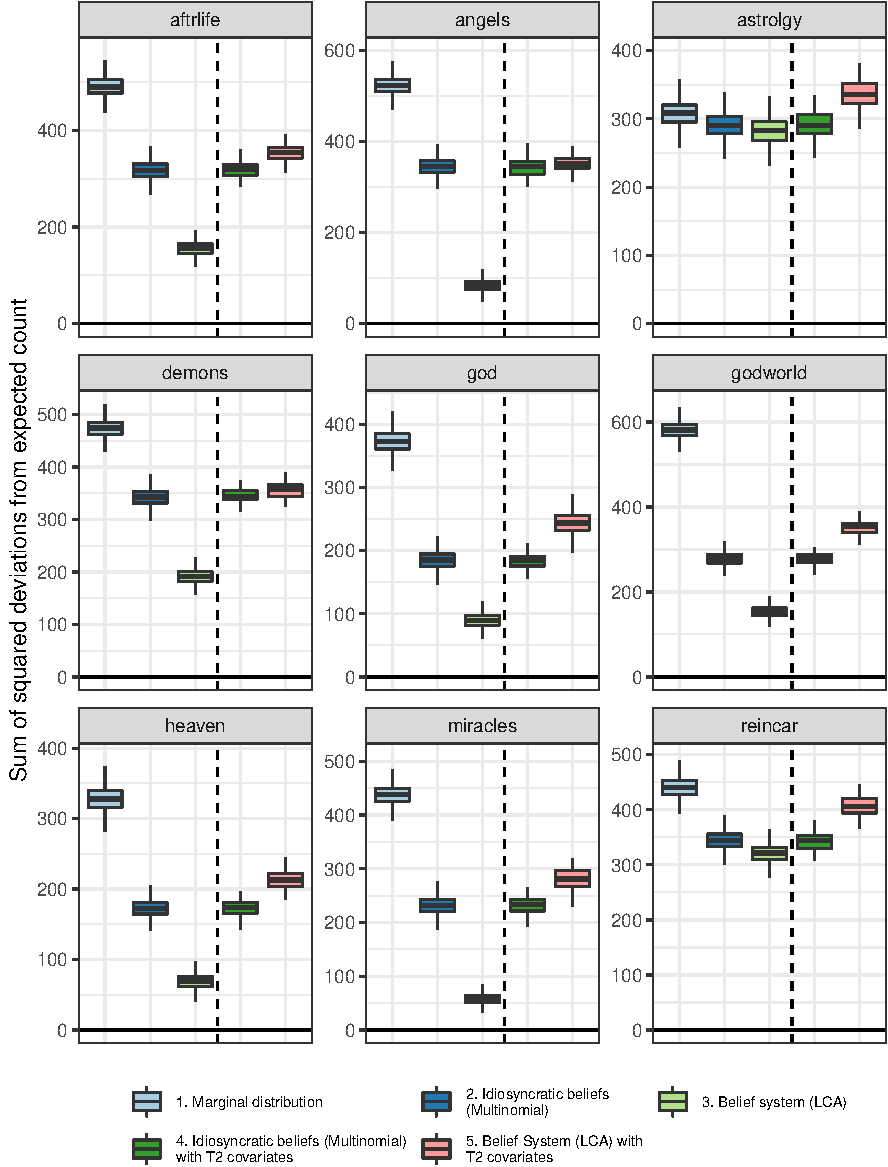
\includegraphics{rethinking_constraint_revision_files/figure-latex/predictionerrorrel-1} 

}

\caption{Boxplots of deviation of observed from expected counts of response patterns, 10,000 iterations each, religious beliefs}\label{fig:predictionerrorrel}
\end{figure}

\begin{verbatim}
## Warning: Removed 1 rows containing non-finite values (stat_boxplot).
\end{verbatim}

\begin{figure}

{\centering 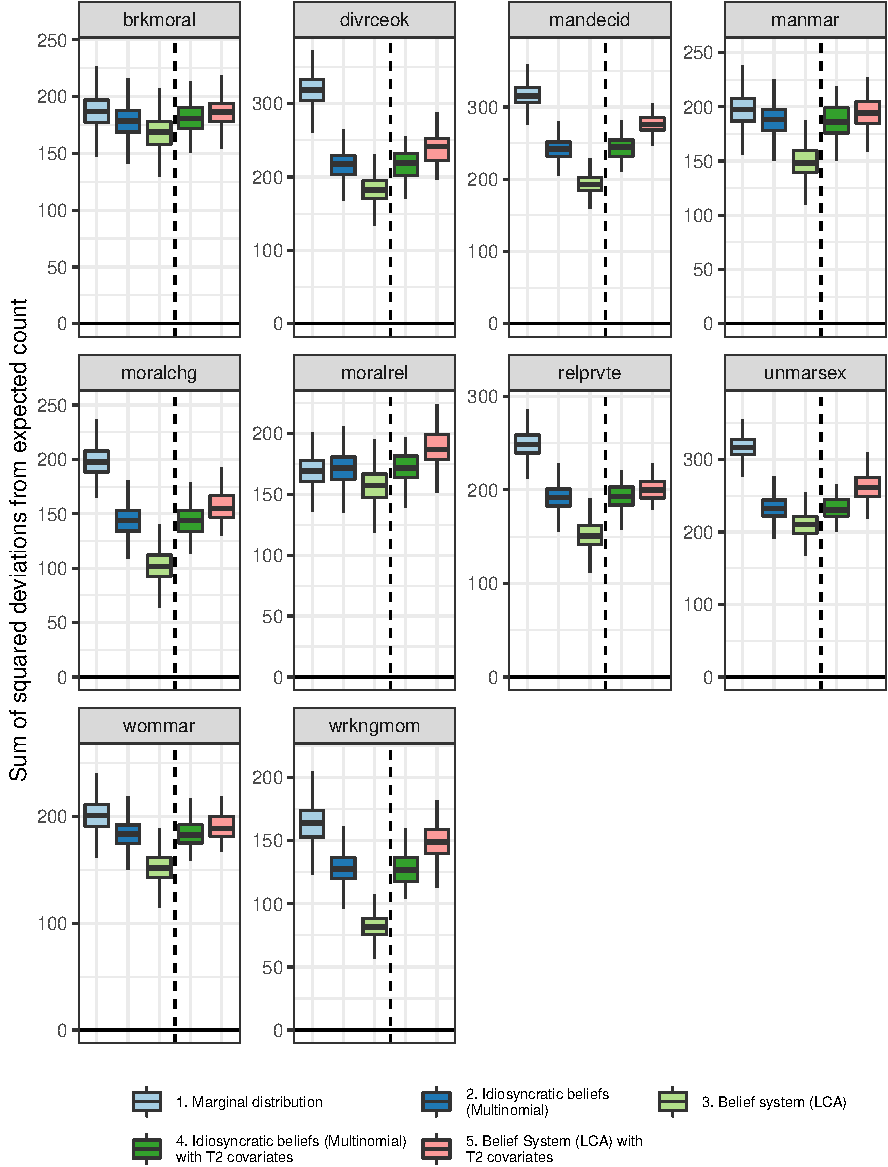
\includegraphics{rethinking_constraint_revision_files/figure-latex/predictionerrornotrel-1} 

}

\caption{Boxplots of deviation of observed from expected counts of response patterns, 10,000 iterations each, moral and family beliefs}\label{fig:predictionerrornotrel}
\end{figure}

The predictions generated through the latent class model consistently outperform the predictions made through the multinomial logit model. For some questions, especially the religious beliefs, differences between the two models is stark, with the belief system model improving prediction substantially over the marginal distribution and the independent beliefs model. Other questions are less conclusive, but the latent class model still tends to outperform the independent beliefs model on average. Unsurprisingly, the model appears to perform best on questions where the five belief systems impose different constraints and worst where belief systems present similar constraints. Because there are not stark differences in the constraints the systems impose around whether it is acceptable to break moral rules for personal gain or belief in astrology, there is not much room for either model to improve upon the marginal distribution.

The key interpretation of this comparison is that information about people's beliefs tell us something about their other beliefs, suggesting an underlying structure to the belief system. The assumption that responses at any wave are a multinomial draw from the distributions deduced at time 1 is well supported, especially for the Christian religious beliefs.

Both the multinomial logit (independent beliefs) and the latent class (belief system) model assume the belief systems that people have, whether idiosyncratic or culturally shared, are durable over time. They cannot adjudicate whether beliefs are principally a result of stable social circumstances or durable cognition. I now turn to adjudicating that question.

\hypertarget{changing-social-circumstances}{%
\subsubsection{Changing Social Circumstances}\label{changing-social-circumstances}}

The final hypothesis explores whether changes organizational participation and social networks better account for changing beliefs than the belief systems explored above. Table \ref{tab:covsum} shows how the organizational participation and social structure variables change between times 1 and 2. There are two notable changes that are likely to produce shifts in beliefs. First, people decrease the amount they attend religious services. Second, there are shifts in religious affiliation. People move out of the indeterminate religion group and the ``no affiliation'' group grows. Since both affiliation and frequency of attendance strongly differentiated the five classes, changes in these variables should produce changes in beliefs under a non-durable cognition model. Parental closeness, and the proportion of one's close friends who share their beliefs remain relatively unchanged.

\begin{table}
\begin{center}
\begin{tabular}{l r r r r r}
\hline
  & Time 1 &  & Time 2 & \\
  & Mean & S.D. & Mean & S.D.\\
\hline
Age & 17.68 & 1.34 & 20.00 & 1.43\\
\\
Frequency of service attendance (0-6) & 2.62 & 2.22 & 2.01 & 2.10\\
Black Protestants & 0.06 &  & 0.07 & \\
Catholic & 0.20 & & 0.17 & \\
Indeterminate Religion & 0.14 &  & 0.04 & \\
Evangelical Protestant & 0.29 &  & 0.30 & \\
Jewish & 0.04 &  & 0.04 & \\
Mainline Protestant & 0.08 &  & 0.11 & \\
No Affiliation & 0.16 &  & 0.24 & \\
Other Religion & 0.02 &  & 0.03 & \\
\\
South & 0.40 & & 0.40 & \\
\\
Years of education & 11.46 & 1.41 & 12.83 & 1.54\\
Parental closeness (1-6) & 5.07 & 0.86 & 5.12 & 0.91\\
Prop. friends share belief & 0.63 & 0.36 & 0.61 & 0.35\\
\hline
\end{tabular}
\caption{Summary statistics for covariates of belief prediction, times 1 and 2}
\label{table:covsum}
\end{center}
\end{table}

To the right side of the dashed line in each plot in Figures Figures \ref{fig:predictionerrorrel} and \ref{fig:predictionerrornotrel} are predictions generated using time 2 covariates. If changing social circumstances lead to changes in attitudes, these models should outperform those that do not.

In general, the time 1 belief system predictions outperform both the idiosyncratic influence model (the multinomial model) that uses time 2 covariates and a model that uses covariates at time 2 to revise membership in belief systems. There is little change in the predictions for the multinomial logit model compared to just using wave 1 covariates, but the latent class model performs worse when we account for changes in social structure.

In other words, a model that assumes attitudes are principally a reflection of current social structures makes worse predictions for people's attitudes than one that assumes no influence of \ldots{} other than what is caused by prior .

\hypertarget{discussion}{%
\section{Discussion}\label{discussion}}

This paper had two related goals. First, it sought to rethink how researchers interested in the measurement of culturally constrained cognition conceptualize and measure the constriants of these belief systems in observational data. Because the cultural structuring of cognition happens well below the level of a survey response, measuring the relationship between responses can produce misleading conclusions about how culturally shaped cognition works. Existing measures of schematic cognition do not fully take into account how culturally patterned cognition might produce variation in survey responses over time that reflect, rather than undermine, those cognitive structures. I argued that Latent Class Analysis could be used to deduce belief systems that manifest as shared probabilities of giving certain responses to different questions over time.

Using LCA, I deduced five belief systems in the population of adolescents surveyed in the NSYR regarding family structure, morality, and religious beliefs. These systems differ in the constraints (and lack of constraints) they place on attitudes. Results from the first three hypothesis tests find that the within-group constraints implied by the model at time 1 are reflected in individuals' change over time. The key finding of this paper is that the response probabilities derived across people at a single point in time provide a remarkably good prediction of how people changed over time.

The five belief systems should not be interpreted as sharply divided ``cultures'' on these issues. These are somewhat porous classifications that represent common patterns of constraints imposed by cognition. Some people have roughly equal probabilities of being assigned to multiple classes. But they do seem to reflect predictable patterns of attitude constraint over time.

As a second goal, the paper sought to adjudicate the relative influence of these cultural-cognitive structures on attitude behavior over time compared to social-structural influences such as social networks and organizational participation. The fourth hypothesis test finds that the constraints (or lack of constraints) present at time 1 better predict the aggregate pattern of responses over time than models that directly root attitudes in contemporaneous social circumstances. Despite competing expectations that changes in organizational participation and social influences should produce changes in beliefs, the constraints deduced at time 1 appear to strongly limit the effect of these changes, especially on religious beliefs and some family beliefs. This suggests that these underlying dispositions are quite durable, even as they produce heterogeneous responses.

\hypertarget{implications}{%
\subsection{Implications}\label{implications}}

The results presented here suggest that people's cognition is more culturally structured and more durable than lots of work supposes. The assumption that durable cognitive processes have to manifest as durable attitudes reflects an implausible assumption about the relationship between cultural schemas and attitudes. Just because attitudes vacillate does not mean that cognition is not being governed by a belief system that is shared and durable. A belief system that produces instability on one question could produce stability on a different one.

Measuring culture is challenging, and measuring culture in the morass that is people's cognition is even harder. For a long time, researchers looked for the signature of shared culture in shared attitudes and stability. But shared culture is often heterogeneous and conflicting, and the product can be shared instability. But that does not make this any less ``culture.'' Taking seriously the measurement of culture means accounting for this instability.

There are undoubtedly more direct measures getting at people's underlying schemas (Hunzaker and Valentino 2019) or the unconscious processes that shape people's cognition (Miles, Charron-Chénier, and Schleifer 2019). But to the exent that researchers want to understand the limits that culture places on people's cognition, LCA appears to do a reasonable job.

The results pose a challenge to how we understand measurement error. The central assumption of measurement error arguments is that people have an underlying position and that inconsistency is inherent in questions, not in people (Alwin 2007; Ansolabehere, Rodden, and Snyder 2008). The theoretical model outlined here builds on previous arguments suggesting people do not have ``attitudes'' or ``beliefs'' as measured by surveys. They have considerations that probabilistically produce responses under a variety of conditions (Zaller 1992). What the latent class analysis shows is that inconsistency is a relationship between people's range of beliefs and the question they answer. Some belief structures strongly constrain people to present consistent responses, but others free people to give a range of attitude reports over time. Moderates, Unconstrained, and Ambivalents have similar average responses on a number of questions. Where they differ is in their variance, but that variance is predicted by their other beliefs, not random error.

Because belief systems appear to be quite durable in the face of changing circumstances, there is no reason to expect that inconsistency in survey responses should be thought of as undermining the causal power of cultural beliefs (Jerolmack and Khan 2014). Inconsistency in survey response should be thought of as reflecting a misalignment between the structures of cognition and the survey question, not reflecting unstructured thought. Studies that find a strong predictive link between survey questions and attitudes might simply get lucky in finding both a question and behaviors that are strongly predicted by a belief system. But better measures of belief systems could potentially show stronger links between these underlying cognitive structures and social action. As Harding (2007) shows, external cultural heterogeneity can predictive of certain kinds of behaviors across domains. Internal cultural heterogeneity might also produce specific lines of behavior. A schematic structure that produces inconsistency on the divorce question potentially causes more divorces than one that constrains beliefs over time to oppose divorce.

Because these cognitive structures appear to be so durable, findings presented here suggest that research focusing on explaining attitude behavior over time might put too much emphasis on contemporary social structures at the expense of cognitive structures formed early in life. In general, people's cognition allows for features of the environment to shape their attitudes. But the range of response possibilities seems to be constrained by cultural-cogntive structures formed early in life. A change in the social environment -- moving from the south to the norteast, for example -- might lead an Unconstrained person to rethink their religious beliefs, but that same change should not affect a Believer. This means that the average effect of some change on an attitude is going to be shaped by who holds what constraints. Without deducing cultural constraints first, however, we might not be able to make sense of this kind of treatment effect.

To be clear, these results should not downplay the role of organizational structures and social networks in shaping people's belief patterns. Organizational participation, especially religious tradition and frequency of religious service attendance, were strong predictors of belief systems at time 1 (and, therefore, beliefs in subsequent waves). These ``past conditions of production'' should be consider particularly important in shaping people's cognition over time (Bourdieu 1990).

Since people do not durably change their attitudes much over time, some researchers have questioned the utility of measuring the same attitudes over time (Kiley and Vaisey 2020). The results presented here suggest that measuring attitudes over time can provide different perspectives on how culture works in people.

\hypertarget{limitations-and-conclusions}{%
\subsection{Limitations and Conclusions}\label{limitations-and-conclusions}}

An important caveat to the above presentation is that Wave 2 of the NSYR -- time 1 in this study -- occurs at what seems to be a particularly formative period in people's life course. Respondents were between the ages of 16 and 20 when they were interviewed for wave 2 of the NSYR. Research suggests that people's attitudes on a range of issues appear to crystallize prior to adulthood (Kiley and Vaisey 2020; Vaisey and Lizardo 2016). This likely strengthens the link between social structures at time 1 and attitudes over time. Time 2 reflects a particularly tumultuous time in people's social structures. If people are in college or newly entered into the workforce, they might have less control over their social structures than they might at other points in the life course. As people settle into adult routines, selecting into new social structures that they have greater control over, we might expect a greater link between these structures and attitudes that what is observed at time 2.

The results presented here suggest that variation in survey responses is not simply random error, but a meaningful reflection of people's social and cultural experiences that is predictable.

\newpage

\hypertarget{references}{%
\section{References}\label{references}}

\singlespace
\setlength{\parindent}{-0.2in}
\setlength{\leftskip}{0.2in}
\setlength{\parskip}{0pt}

\noindent

\hypertarget{refs}{}
\leavevmode\hypertarget{ref-alwin2007}{}%
Alwin, Alwin, Duane F. 2007. \emph{Margins of Error: A Study of Reliability in Survey Measurement}. Hoboken, N.J.: John Wiley \& Sons.

\leavevmode\hypertarget{ref-alwin1991}{}%
Alwin, Duane F., and Jon A. Krosnick. 1991. ``Aging, Cohorts, and the Stability of Sociopolitical Orientations over the Life Span.'' \emph{American Journal of Sociology} 97 (1). University of Chicago Press: 169--95.

\leavevmode\hypertarget{ref-ansolabehere2008}{}%
Ansolabehere, Stephen, Jonathan Rodden, and James M. Snyder. 2008. ``The Strength of Issues: Using Multiple Measures to Gauge Preference Stability, Ideological Constraint, and Issue Voting.'' \emph{American Political Science Review} 102 (2): 215--32. \url{https://doi.org/10.1017/S0003055408080210}.

\leavevmode\hypertarget{ref-baldassarri2008}{}%
Baldassarri, Delia, and Andrew Gelman. 2008. ``Partisans Without Constraint: Political Polarization and Trends in American Public Opinion.'' \emph{American Journal of Sociology} 114 (2): 408--46.

\leavevmode\hypertarget{ref-baldassarri2014}{}%
Baldassarri, Delia, and Amir Goldberg. 2014. ``Neither Ideologues nor Agnostics: Alternative Voters' Belief System in an Age of Partisan Politics.'' \emph{American Journal of Sociology} 120 (1). The University of Chicago Press: 45--95. \url{https://doi.org/10.1086/676042}.

\leavevmode\hypertarget{ref-bartels2014}{}%
Bartels, Larry M., and Simon Jackman. 2014. ``A Generational Model of Political Learning.'' \emph{Electoral Studies} 33 (March): 7--18. \url{https://doi.org/10.1016/j.electstud.2013.06.004}.

\leavevmode\hypertarget{ref-bonikowski2016}{}%
Bonikowski, Bart, and Paul DiMaggio. 2016. ``Varieties of American Popular Nationalism.'' \emph{American Sociological Review} 81 (5). SAGE Publications Inc: 949--80. \url{https://doi.org/10.1177/0003122416663683}.

\leavevmode\hypertarget{ref-bourdieu1990}{}%
Bourdieu, Pierre. 1990. \emph{The Logic of Practice}. Stanford, Calif. : Stanford University Press, 1990.

\leavevmode\hypertarget{ref-boutyline2017}{}%
Boutyline, Andrei. 2017. ``Improving the Measurement of Shared Cultural Schemas with Correlational Class Analysis: Theory and Method.'' \emph{Sociological Science} 4 (May): 353--93. \url{https://doi.org/10.15195/v4.a15}.

\leavevmode\hypertarget{ref-converse1964}{}%
Converse, Philip E. 1964. ``The Nature of Belief Systems in Mass Publics (1964).'' In \emph{Ideology and Discontent}, edited by D. E. Apter, 18:206--61. New York: Free Press.

\leavevmode\hypertarget{ref-dandrade1995}{}%
D'Andrade, Roy G. 1995. \emph{The Development of Cognitive Anthropology}. Cambridge: Cambridge University Press. \url{https://doi.org/10.1017/CBO9781139166645}.

\leavevmode\hypertarget{ref-dellaposta2015}{}%
DellaPosta, Daniel, Yongren Shi, and Michael Macy. 2015. ``Why Do Liberals Drink Lattes?'' \emph{American Journal of Sociology} 120 (5). The University of Chicago Press: 1473--1511. \url{https://doi.org/10.1086/681254}.

\leavevmode\hypertarget{ref-dimaggio1997}{}%
DiMaggio, Paul. 1997. ``Culture and Cognition.'' \emph{Annual Review of Sociology} 23: 263--87.

\leavevmode\hypertarget{ref-dimaggio2018a}{}%
DiMaggio, Paul, Ramina Sotoudeh, Amir Goldberg, and Hana Shepherd. 2018. ``Culture Out of Attitudes: Relationality, Population Heterogeneity and Attitudes Toward Science and Religion in the U.S.'' \emph{Poetics} 68 (June): 31--51. \url{https://doi.org/10.1016/j.poetic.2017.11.001}.

\leavevmode\hypertarget{ref-frye2015}{}%
Frye, Margaret, and Jenny Trinitapoli. 2015. ``Ideals as Anchors for Relationship Experiences.'' \emph{American Sociological Review} 80 (3): 496--525. \url{https://doi.org/10.1177/0003122415581333}.

\leavevmode\hypertarget{ref-ghitza}{}%
Ghitza, Yair, Andrew Gelman, and Jonathan Auerbach. n.d. ``The Great Society, Reagan's Revolution, and Generations of Presidential Voting,'' 21.

\leavevmode\hypertarget{ref-goldberg2011}{}%
Goldberg, Amir. 2011. ``Mapping Shared Understandings Using Relational Class Analysis: The Case of the Cultural Omnivore Reexamined.'' \emph{American Journal of Sociology} 116 (5). The University of Chicago Press: 1397--1436. \url{https://doi.org/10.1086/657976}.

\leavevmode\hypertarget{ref-goldberg2018}{}%
Goldberg, Amir, and Sarah K. Stein. 2018. ``Beyond Social Contagion: Associative Diffusion and the Emergence of Cultural Variation.'' \emph{American Sociological Review} 83 (5). SAGE Publications Inc: 897--932. \url{https://doi.org/10.1177/0003122418797576}.

\leavevmode\hypertarget{ref-goodman1974}{}%
GOODMAN, LEO A. 1974. ``Exploratory Latent Structure Analysis Using Both Identifiable and Unidentifiable Models.'' \emph{Biometrika} 61 (2): 215--31. \url{https://doi.org/10.1093/biomet/61.2.215}.

\leavevmode\hypertarget{ref-harding2007}{}%
Harding, David J. 2007. ``Cultural Context, Sexual Behavior, and Romantic Relationships in Disadvantaged Neighborhoods.'' \emph{American Sociological Review} 72 (3): 341--64. \url{https://doi.org/10.1177/000312240707200302}.

\leavevmode\hypertarget{ref-hill2001a}{}%
Hill, Jennifer L., and Hanspeter Kriesi. 2001. ``An Extension and Test of Converse's "Black-and-White" Model of Response Stability.'' \emph{The American Political Science Review} 95 (2). {[}American Political Science Association, Cambridge University Press{]}: 397--413.

\leavevmode\hypertarget{ref-hofman2017}{}%
Hofman, Jake M., Amit Sharma, and Duncan J. Watts. 2017. ``Prediction and Explanation in Social Systems.'' \emph{Science} 355 (6324). American Association for the Advancement of Science: 486--88. \url{https://doi.org/10.1126/science.aal3856}.

\leavevmode\hypertarget{ref-hout2016}{}%
Hout, Michael, and Orestes P. Hastings. 2016. ``Reliability of the Core Items in the General Social Survey: Estimates from the Three-Wave Panels, 2006--2014.'' \emph{Sociological Science} 3 (November): 971--1002. \url{https://doi.org/10.15195/v3.a43}.

\leavevmode\hypertarget{ref-hunzaker2016}{}%
Hunzaker, M. B. Fallin. 2016. ``Cultural Sentiments and Schema-Consistency Bias in Information Transmission.'' \emph{American Sociological Review} 81 (6): 1223--50. \url{https://doi.org/10.1177/0003122416671742}.

\leavevmode\hypertarget{ref-hunzaker2019}{}%
Hunzaker, M.B. Fallin, and Lauren Valentino. 2019. ``Mapping Cultural Schemas: From Theory to Method.'' \emph{American Sociological Review} 84 (5). SAGE Publications Inc: 950--81. \url{https://doi.org/10.1177/0003122419875638}.

\leavevmode\hypertarget{ref-jerolmack2014}{}%
Jerolmack, Colin, and Shamus Khan. 2014. ``Talk Is Cheap: Ethnography and the Attitudinal Fallacy.'' \emph{Sociological Methods \& Research} 43 (2): 178--209. \url{https://doi.org/10.1177/0049124114523396}.

\leavevmode\hypertarget{ref-kahneman2011}{}%
Kahneman, Daniel. 2011. \emph{Thinking, Fast and Slow}. New York: Farrar, Straus and Giroux.

\leavevmode\hypertarget{ref-kiley2020}{}%
Kiley, Kevin, and Stephen Vaisey. 2020. ``Measuring Stability and Change in Personal Culture Using Panel Data.'' \emph{American Sociological Review} 85 (3). SAGE Publications Inc: 477--506. \url{https://doi.org/10.1177/0003122420921538}.

\leavevmode\hypertarget{ref-kinder2017}{}%
Kinder, Donald R., and Nathan P. Kalmoe. 2017. \emph{Neither Liberal nor Conservative: Ideological Innocence in the American Public}. Chicago: University of Chicago Press.

\leavevmode\hypertarget{ref-lazarsfeld1968}{}%
Lazarsfeld, Paul F., and Neil W. Henry. 1968. \emph{Latent Structure Analysis}. 1st edition. Houghton Mifflin Company.

\leavevmode\hypertarget{ref-lewis2018}{}%
Lewis, Kevin, and Jason Kaufman. 2018. ``The Conversion of Cultural Tastes into Social Network Ties.'' \emph{American Journal of Sociology} 123 (6): 1684--1742. \url{https://doi.org/10.1086/697525}.

\leavevmode\hypertarget{ref-lizardo2006}{}%
Lizardo, Omar. 2006. ``How Cultural Tastes Shape Personal Networks.'' \emph{American Sociological Review} 71 (5): 778--807. \url{https://doi.org/10.1177/000312240607100504}.

\leavevmode\hypertarget{ref-lizardo2010a}{}%
Lizardo, Omar, and Michael Strand. 2010. ``Skills, Toolkits, Contexts and Institutions: Clarifying the Relationship Between Different Approaches to Cognition in Cultural Sociology.'' \emph{Poetics} 38 (2): 205--28. \url{https://doi.org/10.1016/j.poetic.2009.11.003}.

\leavevmode\hypertarget{ref-martin2002}{}%
Martin, John Levi. 2002. ``Power, Authority, and the Constraint of Belief Systems.'' \emph{American Journal of Sociology} 107 (4): 861--904. \url{https://doi.org/10.1086/343192}.

\leavevmode\hypertarget{ref-martin2010}{}%
---------. 2010. ``Life's a Beach but You're an Ant, and Other Unwelcome News for the Sociology of Culture.'' \emph{Poetics} 38 (2): 229--44. \url{https://doi.org/10.1016/j.poetic.2009.11.004}.

\leavevmode\hypertarget{ref-mccutcheon1987}{}%
McCutcheon, Allan L. 1987. \emph{Latent Class Analysis}. SAGE. \url{http://books.google.com?id=9J9pyAEACAAJ}.

\leavevmode\hypertarget{ref-miles2015}{}%
Miles, Andrew. 2015. ``The (Re)Genesis of Values: Examining the Importance of Values for Action.'' \emph{American Sociological Review} 80 (4): 680--704. \url{https://doi.org/10.1177/0003122415591800}.

\leavevmode\hypertarget{ref-miles2019}{}%
Miles, Andrew, Raphaël Charron-Chénier, and Cyrus Schleifer. 2019. ``Measuring Automatic Cognition: Advancing Dual-Process Research in Sociology.'' \emph{American Sociological Review} 84 (2). SAGE Publications Inc: 308--33. \url{https://doi.org/10.1177/0003122419832497}.

\leavevmode\hypertarget{ref-mohr1998}{}%
Mohr, John W. 1998. ``Measuring Meaning Structures.'' \emph{Annual Review of Sociology} 24 (1): 345--70. \url{https://doi.org/10.1146/annurev.soc.24.1.345}.

\leavevmode\hypertarget{ref-mohr2020}{}%
Mohr, John W., Christopher A. Bail, Margaret Frye, Jennifer C. Lena, Omar Lizardo, Terence E. McDonnell, Ann Mische, Iddo Tavory, and Frederick F. Wherry. 2020. \emph{Measuring Culture}. Columbia University Press.

\leavevmode\hypertarget{ref-perrin2011}{}%
Perrin, Andrew J., and Katherine McFarland. 2011. ``Social Theory and Public Opinion.'' \emph{Annual Review of Sociology} 37 (1): 87--107. \url{https://doi.org/10.1146/annurev.soc.012809.102659}.

\leavevmode\hypertarget{ref-rawlings2020}{}%
Rawlings, Craig M. 2020. ``Cognitive Authority and the Constraint of Attitude Change in Groups.'' \emph{American Sociological Review} 85 (6). SAGE Publications Inc: 992--1021. \url{https://doi.org/10.1177/0003122420967305}.

\leavevmode\hypertarget{ref-salganik2020}{}%
Salganik, Matthew J., Ian Lundberg, Alexander T. Kindel, Caitlin E. Ahearn, Khaled Al-Ghoneim, Abdullah Almaatouq, Drew M. Altschul, et al. 2020. ``Measuring the Predictability of Life Outcomes with a Scientific Mass Collaboration.'' \emph{Proceedings of the National Academy of Sciences} 117 (15). National Academy of Sciences: 8398--8403. \url{https://doi.org/10.1073/pnas.1915006117}.

\leavevmode\hypertarget{ref-sears1999}{}%
Sears, David O., and Carolyn L. Funk. 1999. ``Evidence of the Long-Term Persistence of Adults' Political Predispositions.'' \emph{The Journal of Politics} 61 (1): 1--28. \url{https://doi.org/10.2307/2647773}.

\leavevmode\hypertarget{ref-smith2005}{}%
Smith, Sandra Susan. 2005. ```Don't Put My Name on It': Social Capital Activation and Job‐Finding Assistance Among the Black Urban Poor.'' \emph{American Journal of Sociology} 111 (1): 1--57. \url{https://doi.org/10.1086/428814}.

\leavevmode\hypertarget{ref-steensland2000}{}%
Steensland, Brian, Jerry Z. Park, Mark D. Regnerus, Lynn D. Robinson, W. Bradford Wilcox, and Robert D. Woodberry. 2000. ``The Measure of American Religion: Toward Improving the State of the Art.'' \emph{Social Forces} 79 (1). Oxford University Press: 291--318. \url{https://doi.org/10.2307/2675572}.

\leavevmode\hypertarget{ref-strauss1998}{}%
Strauss, Claudia, and Naomi Quinn. 1998. \emph{A Cognitive Theory of Cultural Meaning}. Publications of the Society for Psychological Anthropology. Cambridge: Cambridge University Press. \url{https://doi.org/10.1017/CBO9781139167000}.

\leavevmode\hypertarget{ref-swidler1986}{}%
Swidler, Ann. 1986. ``Culture in Action: Symbols and Strategies.'' \emph{American Sociological Review} 51 (2): 273. \url{https://doi.org/10.2307/2095521}.

\leavevmode\hypertarget{ref-swidler2001}{}%
---------. 2001. \emph{Talk of Love: How Culture Matters}. Chicago: University of Chicago Press.

\leavevmode\hypertarget{ref-vaisey2010}{}%
Vaisey, S., and O. Lizardo. 2010. ``Can Cultural Worldviews Influence Network Composition?'' \emph{Social Forces} 88 (4): 1595--1618. \url{https://doi.org/10.1353/sof.2010.0009}.

\leavevmode\hypertarget{ref-vaisey2009}{}%
Vaisey, Stephen. 2009. ``Motivation and Justification: A Dual‐Process Model of Culture in Action.'' \emph{American Journal of Sociology} 114 (6): 1675--1715. \url{https://doi.org/10.1086/597179}.

\leavevmode\hypertarget{ref-vaisey2016}{}%
Vaisey, Stephen, and Omar Lizardo. 2016. ``Cultural Fragmentation or Acquired Dispositions? A New Approach to Accounting for Patterns of Cultural Change.'' \emph{Socius} 2 (January). SAGE Publications: 2378023116669726. \url{https://doi.org/10.1177/2378023116669726}.

\leavevmode\hypertarget{ref-zaller1992}{}%
Zaller, John. 1992. \emph{The Nature and Origins of Mass Opinion}. Cambridge Studies in Public Opinion and Political Psychology. Cambridge: Cambridge University Press. \url{https://doi.org/10.1017/CBO9780511818691}.

\end{document}
